% This document provides the style to be used for a MSc Thesis at the
% Parallel and Distributed Systems group
\documentclass[11pt,twoside,a4paper,openright]{report}

% use babel for proper hyphenation
\usepackage[british]{babel}
\usepackage{graphicx}
\graphicspath{{../figures/}}
\usepackage{url}
\usepackage[noend]{algpseudocode} 
\usepackage{amsmath}
\usepackage{amssymb}
\usepackage{amsthm}
\usepackage{subcaption}
\usepackage{rotating}
\usepackage{framed}
\usepackage{csquotes}
\usepackage[style=numeric]{biblatex}
% \usepackage{times}

% https://tex.stackexchange.com/questions/42343/how-to-add-a-navigation-window-to-a-latex-generated-pdf-document
\usepackage{hyperref}
\hypersetup{pdftex,colorlinks=true,allcolors=blue}
\usepackage{hypcap}

% https://tex.stackexchange.com/questions/1863/which-packages-should-be-loaded-after-hyperref-instead-of-before
\usepackage{cleveref}  
\usepackage{algorithm}


\addbibresource{references.bib} 
\algnewcommand\algorithmicupon{\textbf{Upon}}
\algnewcommand\Upon{\item[\algorithmicupon]}

\algnewcommand\algorithmicsend{\textbf{Send}}
\algnewcommand\Send{\item[\algorithmicsend]}

\DeclareMathOperator*{\argmin}{arg\,min}
\newtheorem{theorem}{Theorem}
\newtheorem{corollary}{Corollary}
\newtheorem{lemma}{Lemma}
\newtheorem{claim}{Claim}
\newtheorem{definition}{Definition}

\newcommand{\A}{\mathcal{A}}
\newcommand{\C}{\mathcal{C}}
\renewcommand{\P}{\mathcal{P}}
\newcommand{\F}{\mathcal{F}}
\newcommand{\E}{\mathcal{E}}

%use this command when you want the next content to appear on an odd page
\newcommand{\clearemptydoublepage}{
    \newpage{\pagestyle{empty}
    \cleardoublepage}
}

\begin{document}

%%%%%%%%%%%%%%%%%%%%%%%%%%%%%%%%%%%%%%%%%%%%%%%%%%%%%%%%%%%%%%%%%%%%%%%%%%%%%%%
\hoffset=1.63cm
\oddsidemargin=0in
\evensidemargin=0in
\textwidth=5in

%%%%%%%%%%%%%%%%%%%%%%%%%%%%%%%%%%%%%%%%%%%%%%%%%%%%%%%%%%%%%%%%%%%%%%%%%%%%%%%
\parindent=1em

\pagestyle{empty}

% FRONTCOVER
\begin{titlepage}

\null\vfill

\begin{center}
\LARGE{TODO TITLE}
\end{center}

\vspace{1.5cm}

\begin{center}
Kelong Cong
\end{center}

\vfill

\begin{figure}[!b]
\centering

\includegraphics[width={0.6\textwidth}]{logo}
\end{figure}

\vspace{2.0cm}

\end{titlepage}



% EMPTY PAGE
\cleardoublepage

\pagestyle{plain}

% TITLE PAGE: page i (hidden)
\begin{titlepage}
\begin{center}

\includegraphics[height=4cm]{figures/logo}\\
%\LARGE
%Delft University of Technology \\
\large
Faculty Electrical Engineering, Mathematics and Computer Science

\vspace*{12cm}

\setlength{\TPHorizModule}{1mm}
\setlength{\TPVertModule}{\TPHorizModule}
% Set the Paragraph Indent to zero, so the first line is not Indented
% Back-up the current value so it can be put back at the end of the title page
\newlength{\backupparindent}
\setlength{\backupparindent}{\parindent}
\setlength{\parindent}{0mm}			
% Begins a textbox at 72 mm from the left of the edge of the paper and 89 mm from the top
% The width of the textbox is 95 mm (167 - 72 mm)
% The height of the box cannot be defined, so it is your task to keep the text not too long
\begin{textblock}{95}(62,89)
    \vspace*{7mm}
    \huge
    \textbf{\doctitle \\}
    \Large
    \vspace*{3mm}
    \textit{\docsubtitle}\\
    \vspace*{10mm}
    \Large
    \me\\
\end{textblock}

\large
Supervisors:\\
\begin{tabular}{rl}
    \firstCommitteeMember\\
    \secondCommitteeMember\\
    \thirdCommitteeMember\\
\end{tabular}

\vfill
\version

\vfill
%\docdate \\
\large
Delft, \monthYear\\

% Put the Paragraph Indent back to its original value
\setlength{\parindent}{\backupparindent}
\end{center}
\end{titlepage} 


% GRADUATION DATA AND ABSTRACT: pages ii and iii (hidden)
%De aankondiging bevat de spreker, titel, plaats, datum en tijd, samenstelling van de afstudeercommissie en een korte samenvatting (maximaal 25 regels).
\thispagestyle{empty}

\noindent \textbf{Author}\\
\begin{tabular}{l}
Kelong Cong\\
\\
\end{tabular}\\
\noindent \textbf{Title}\\
\begin{tabular}{l}
A Blockchain Consensus Protocol With Horizontal Scalability\\
\\
\end{tabular}\\
\noindent \textbf{MSc presentation}\\
\begin{tabular}{l}
% <MM> DD, YYYY (like \today)
31st August 2017\\
\\
\end{tabular}

\vspace{1.1cm}

\noindent \textbf{Graduation Committee}\\
\begin{tabular}{ll}
% The order of listing the names: Graduation prof, supervisor(s), others ordered by title + alphabetical
%examples:
Prof. dr. ir. D. H. J. Epema            & Delft University of Technology \\
Dr. ir. J. A. Pouwelse                  & Delft University of Technology \\
Dr. Z. Erkin                            & Delft University of Technology \\
\end{tabular}

\begin{abstract}
% what's the problem?
Blockchain systems have the potential to decentralise many traditionally centralised systems.
However, scalability remains a key challenge.
Without a horizontally scalable solution, blockchain systems remain unsuitable for ubiquitous use.
% what's the solution?
We design a novel blockchain system called \textsc{Checo}.
Each node in our system maintains a personal hash chain,
which only stores transactions that the node is involved in.
A consensus is reached on special blocks called checkpoint blocks rather than on all the transactions.
Checkpoint blocks are effectively a hash pointer to the personal hash chains,
thus a single checkpoint block may represent a large set of transactions.
The consensus protocol does not imply transaction validity.
Hence we introduce a validation protocol which allows nodes to verify that the transactions are correctly recorded,
meaning that consensus on transactions is achieved indirectly via checkpoint blocks.
% how good is the solution?
We evaluate \textsc{Checo} analytically and experimentally.
Our results show a strong indication of horizontal scalability even in the worst case,
where every transaction is made with a randomly selected node.
\end{abstract}

\clearpage



\pagenumbering{roman}
\setcounter{page}{4}

% EMPTY PAGE: page iv
\cleardoublepage

% OPTIONAL QUOTATION: page v
%\pagestyle{empty}

\null\vfill

\begin{center}
\emph{``TODO QUOTE''} -- TODO QUOTED PERSON
\end{center}

\vspace{10cm}

\clearpage


% EMPTY PAGE: page vi
%\cleardoublepage

% PREFACE: page v
\chapter*{Preface}
\addcontentsline{toc}{chapter}{Preface}
TODO MOTIVATION FOR RESEARCH TOPIC

\vspace{1\baselineskip}

\noindent
TODO ACKNOWLEDGEMENTS

\vspace{1\baselineskip}

\noindent
TODO AUTHOR

\vspace{1\baselineskip}

\noindent
Delft, The Netherlands

\noindent
\today

% EMPTY PAGE: page vi
\cleardoublepage

% TABLE OF CONTENTS: starting at page vii
\tableofcontents

\cleardoublepage

\pagenumbering{arabic}
\setcounter{page}{1}

This is a story about a scalable blockchain framework and Byzantine
generals\dots

%%% Local Variables:
%%% mode: latex
%%% TeX-master: "../thesis"
%%% End:
\clearemptydoublepage

\chapter{Problem description}
\label{ch:problem}

From the Introduction, we saw that early blockchain systems face a scalability problem.
In particular, the use proof-of-work is unlikely to reach a transaction rate suitable for ubiquitous use.
Many attempts to fix the scalability problem exist in academia as well as the industry.
In this chapter, we describe the related work in the form of a mini taxonomy and identify areas for improvement and limitations.
Then we state our research question which aims to overcome some of the limitations.

\section{Related work and mini taxonomy}
\label{sec:taxonomy}

Blockchain research has seen a surge in recent years from both the industry and academia,
this resulted in a myriad of blockchain systems with different approaches to scalability.
To understand the current state-of-the-art,
we classify various blockchain systems by their scalability approach.

\subsection{Early blockchain systems}
This category represents the baseline,
which are systems with a probabilistic consensus algorithm.
That is, transactions never reach consensus with a probability of 1.
Given sufficient computational power, adversaries are able to undo any transaction.
The typical examples are proof-of-work based systems such as Bitcoin, Ethereum and other Altcoins.
In Bitcoin, nodes compete in solving puzzles.
The first node solves the puzzle has the privilege to create a new block.
The level of consensus of a block containing many transactions is determined by how deep it is in the Bitcoin blockchain,
also called the number of confirmation.
The probability of a block being orphaned drops exponentially as the depth increases~\cite{bitcoin}.
Nevertheless, the probability of the highest block being orphaned is non-negligible.

The advantage of this approach is that it can be used in a large network.
In fact, prior to Bitcoin, there was no internet-scale consensus protocol.
Bitcoin is also fault-tolerant because attackers can not out pace honest users in finding new blocks unless they have a majority of the hash power.
As long as the majority is honest and reasonable measures are taken to prevent the selfish mining attack~\cite{eyal2014majority}.
The disadvantage, however, is that transactions are never in consensus with a probability of 1---no consensus finality.
Hence double spending is possible for transactions that do not have a large number of confirmations.
Furthermore, as we mentioned in the~\Cref{ch:intro},
the performance is limited due to the fact that blocks are of fixed size and are generated at fixed intervals.
Thus early blockchain systems do not achieve horizontal scalability.

% Our system significantly improves upon Bitcoin and other classical blockchain systems in performance, scalability and consensus finality.
% The results described in \Cref{ch:analysis} and \Cref{ch:implementation}, show that we have horizontal scalability,
% where more nodes result in more global throughput.
% Further, we do not have the aforementioned probabilistic behaviour,
% once some consensus result is decided, it cannot be orphaned, thus our consensus is final.
% The leadership election is also not ideal in classical blockchain systems.
% Mining can be seen as a technique to elect a single leader.
% The leader has full control of what goes into the block thus it may selectively censor transactions.
% We use ACS, so as long as the CP block is in $n - 2t$ nodes, it is guaranteed to be in consensus.

% However, the security aspect falls short of the ``honest majority'' security model that classical blockchains claim to 
% have\footnote{Recently it was shown that doing selfish-ming would give the adversary an unfair advantage when she only controls 25\% of the mining power~\cite{eyal2014majority}}.
% Our system risks going into erroneous state if the inequality $n \ge 3t + 1$ is not satisfied.
% Classical blockchain systems also have an incentive mechanism, thus they do not depend on altruistic nodes and encourages participation.
% Our system on the other hand does not have an incentive mechanism because we make no assumptions on the application.

\subsection{Off-chain transactions and payment networks}
Off-chain transactions make use of the following fact.
If nodes make frequent transactions,
then it is not necessary to store every transaction on the blockchain,
only the net settlement is necessary.
The best examples are Lightning Network~\cite{lightningnetwork} and Duplex Micropayment Channels~\cite{decker2015fast}.

Off-chain transaction systems are implemented using multi-signature addresses~\cite{bitcoinmultisig} and hashed time-locked Bitcoin contracts~\cite{bitcointimelock}.
In the simplest case, 
if two parties wish to make transactions,
they open a payment channel in the form of a multi-signature Bitcoin address (for two parties it would be a 2-of-2 signature address).
Each of the party must also deposit some Bitcoins in the multi-signature address,
this is called the opening transaction.
Both parties keep the channel state which is not broadcasted to the network.
The state is updated when the two parties make new transactions.
The protocol disincentivises the parties from broadcasting old channel states.
If this occurs, the counterparty can drain all the Bitcoins in the channel.
To close the channel, the parties simply broadcast the latest net settlement to the Bitcoin network,
this is called the closing transaction.
Effectively, only two transactions need to be broadcasted to the Bitcoin network---the opening and the closing transaction,
even if the two parties made thousands or millions of transactions in between.
The two-party scheme can be extended to a network of channels,
which allows two parties to make off-chain transactions without an open channel as long as they are connected by nodes that do.

The advantage of such systems is that they act as add-ons to Bitcoin wish already has a large number of users.
Thus, if enough of the network wish for it (by setting a new block version),
then a large number of users will instantly benefit from it.
Some implementations already exist\footnote{For example \url{https://github.com/lightningnetwork/lnd}.},
but at the time of writing SegWit is not activated yet which is a prerequisite for Lightning Network.

On the other hand, payment channel complicates user experience and leads to centralisation.
As we mentioned earlier, each node must deposit some Bitcoins into a multi-signature account.
The users must pick a suitable amount.
If the deposit is too low it would not allow large transactions.
If the deposit is too high the user is locked out of much of its Bitcoins for use outside of the channel.
In addition, the user must proactively check whether the counterparty has broadcasted an old channel state so that the user does not lose Bitcoins.
Furthermore, creating channels with sufficient balance and also keeping it online to act as a router is expensive.
A casual user is not capable of such tasks, thus it leads to centralisation.
Payment channels, in theory, solve the scalability problem of early blockchain systems,
but to the best of our knowledge, its exact scalability characteristics are not investigated.

% Further, off-chain transactions are limited only to an exchange of cryptocurrency,
% it is less general than typical Bitcoin transactions which may be a simple smart contract.
% Time-locked contracts have a strong dependency on timing, thus disputes may arise when the payment channel is just about to close.
% Our system is purely asynchronous and make no assumption on timing,
% in fact we assume the adversary has control of the message delivery time and order.


\subsection{Permissioned systems based on Byzantine consensus}

This category of systems uses traditional Byzantine consensus algorithms such as PBFT~\cite{castro1999practical}.
In essence, they contain a fixed set of nodes (sometimes called validating peer) that run a Byzantine consensus algorithm to decide on new blocks.
This technique is often used in permissioned system where the validators must be predetermined.
For example, Hyperledger Fabric~\cite{cachin2016architecture}.

A nice aspect of Byzantine consensus and in particular PBFT is that it can handle much more transactions than classical blockchain systems.
PBFT can, for example, achieve 10,000 TX/s if the number of validating peer is under 16~\cite[Section 5.2]{miller2016honey}.
Further, in contrast to proof-of-work, PBFT consensus is final.
That is, transaction history cannot be re-written if it is already in the blockchain.

The major drawback of Byzantine consensus based systems is that it does not scale in terms of the number of validating peers.
Going back to PBFT, its transaction rate drops to under 5000 TX/s when the number of validating peer is 64~\cite[Section 5.2]{miller2016honey}.
Moreover, the validating peers are predetermined which makes the system unsuitable for the open internet.

% But our system has the potential to perform beyond that of PBFT because we represent many transactions with a single CP block,
% enabling horizontal scalability.
% Furthermore, since PBFT relies on a leader, it is not censorship resiliant.
% Our system on the other hand has the benifits of ACS where CP blocks cannot be censored.
% Finally, our system is able to work in the permissionless setting by simply submitting new CP blocks to the facilitators.
% It can even be adapted to work in the permissioned by simply removing the luck value computation.

% What we wish to have which is in Hyperledger is a smart contract system (also known as chaincodes in Hyperledger).
% We hope to design and implement smart contracts by adding additional logic to the transaction protocol and the validation protocol.
% Such functionalities we believe is better to be built into the backbone rather than having it as an add on.

\subsection{Combining proof-of-work with Byzantine consensus}
Recent research has developed a class of hybrid systems which uses PoW for committee election,
and Byzantine consensus algorithms to agree on transactions.
This design is primarily for permissionless system because the PoW leader election aspect prevents Sybils.
% And then they use a Byzantine consensus algorithm to actually reach consensus on a set of transactions within the committee.
Some examples are SCP~\cite{luu2015scp}, ByzCoin~\cite{kogias2016enhancing} and Solidus~\cite{abraham2016solidus}.

This technique overcomes the early blockchain scalability issue by delegating the transaction validation to the Byzantine consensus protocol (e.g., PBFT in ByzCoin~\cite{kogias2016enhancing}).
A major tradeoff of such systems is that they cannot guarantee correctness when there is a large number of malicious nodes (but less than a majority).
For SCP, ByzCoin and Solidus, they all have some probability to elect more than $t$ Byzantine nodes into the committee,
where $t$ is typically just under a third of the committee size (a lower bound of Byzantine consensus~\cite{pease1980reaching}).
This problem is especially difficult to solve because the committee is always much smaller than the population size which has more than $t$ Byzantine nodes.
Classical blockchain does not have this problem because they do not use Byzantine consensus.
Further, due to the fact that these systems must reach consensus on all transactions, none of them achieves horizontal scalability.

\subsection{Sharding}

Sharding is a technique to achieve horizontal scalability by grouping nodes into multiple committees or shards.
Nodes within a single shard run a Byzantine consensus algorithm to agree on a set of transactions that belong to that specific shard.
An intra-shard protocol is needed for transactions that involve nodes from more than one shard.
The number of shards grows linearly with respect to the total computational power in the network.
This scheme achieves horizontal scalability because if every shard commits transactions at the same throughput,
then adding more shard would naturally result in a linear increase of global throughput.
Examples of blockchain systems that use sharding are Elastico~\cite{luu2016elastico} and OmniLedger~\cite{kokoris2017omniledger}.

The biggest limitation of sharding is that it is only optimal is transactions stay in the same shard.
In fact, Elastico cannot atomically process inter-shard transactions.
OmniLedger has an inter-shard transaction protocol but choosing a good shard size is difficult.
A large shard size would make the system less scalable because the Byzantine consensus algorithm must be run by a large number of nodes.
A small shard size would result in a large number of inter-shard transactions which also hinder scalability.
The authors of OmniLedger noted that inter-shard transactions have significantly higher latency compared to the consensus protocol~\cite{kokoris2017omniledger}.
Furthermore, since no shards can be compromised for the system to function correctly,
the adversaries have more opportunities to compromise the system.

\subsection{Blockchain without global consensus}

Tangle~\cite{tangle}, Corda~\cite{corda} and the original TrustChain~\cite{multichain} do not use global consensus at all.
In this scheme, every node has their own chain.
Transactions between nodes are recorded on their respective chains.
This effectively results in a directed acyclic graph.
By avoiding global consensus, this approach achieves extremely desirable scalability properties similar to BitTorrent~\cite{cohen2003incentives}.

On the other hand, the application and security are limited.
A malicious node can easily lie to other nodes regarding its own chain by simply presenting one version of reality to a set of nodes and another version to a different set.
Thus the network will have a conflicting view on the state of the malicious node.
Applications such as digital cash can not be implemented on top of such systems because consistency is needed in solving the double spending problem.

% Our system can be considered as the same as these types of blockchains but with a lightweight consensus protocol.
% Consensus might not be applicable in all applications.
% But we believe it is important for detecting and preventing fraud.
% The example in~\Cref{fig:trustchain-bad} on page~\pageref{fig:trustchain-bad} demonstrates this.
% If $b$ makes a fork and $a$ and $c$ have no way to communicate (e.g. the adversary may control parts of the network) ,
% then $c$ is tricked to believe that her transaction with $b$ is valid.
% Only when $c$ sees a conflicting chain is she able to tell that the transaction is invalid.
% But $c$ does not know the true end-of-chain of $b$, thus she can never know whether her transaction is valid.
% This is not possible in our system because $b$ cannot convince $c$ unless he can compute exponential time algorithms
% (this is finding the second preimage for a hash function).

% However, consensus and validation comes at a cost that do not exist in Tangle, Corda or the original TrustChain.
% Our transaction rate is affected by the validation protocol in the worst case scenario as we saw in~\Cref{sec:evaluation}.

\section{Research question}

We saw in~\Cref{sec:taxonomy} that the majority of the systems cannot achieve horizontal scalability.
To the best of our knowledge, only two systems---Elastico~\cite{luu2016elastico} and OmniLedger~\cite{kokoris2017omniledger}---has experimentally demonstrated horizontal scalability.
However, these techniques rely on sharding, thus the performance highly depends on transaction characteristics and the shard size parameter because inter-shard transactions are slow.
Furthermore, all the systems described in~\Cref{sec:taxonomy} are complete blockchain systems designed for a concrete application.
We wish to design a blockchain consensus protocol that can be used in many applications.
For example, the accounting of detailed internet traffic in Tribler~\cite{pouwelse2008tribler, multichain} and decentralised market\footnote{\url{https://github.com/Tribler/tribler/blob/devel/Tribler/community/tradechain/__init__.py}}.
Hence our research question is the following.
\begin{displayquote}
\emph{How can we design a blockchain consensus protocol that is fault-tolerant,
horizontally scalable,
and able to reach global consensus?}
\end{displayquote}

In order to make sense of our research question, we must first define \emph{blockchain consensus protocol}.
Typical blockchain systems are application specific.
For example, the application in Bitcoin (any many of its derivatives) is digital cash, the application in Namecoin is domain name registration~\cite{namecoin} and the application in Siacoin is cloud storage~\cite{siacoin}.
Underneath these applications lies the blockchain consensus protocol which has the goal of reaching consensus on transactions or state changes.
In the case of Bitcoin, it is proof-of-work (PoW).
It is not concerned with the structure of the transactions,
it works by simply treating transactions as a blob of data and hashes them with the previous block.
In this work, we focus on the blockchain consensus protocol rather than any specific application.
Because it is the scalability bottleneck and is necessary for any blockchain based application.
% Also, it should be possible to build any kind of application on top our system.
% We do not impose on a consensus algorithm, as long as it satisfies the properties of atomic broadcast which we describe in~\Cref{sec:overview-cons}.

In the remainder of this section, we expand on our research question and visit each of our requirements in detail.
At the end of this section, we describe some issues that we do not consider as a part of our design,
which is the result of not focusing on any specific application.

\subsection*{Global consensus}
% WHY WE NEED GLOBAL CONSENSUS?
Having consensus is essential in blockchain systems.
It stops many types of malicious activities because the agreed state, or a representation of it, must have the consent of the honest nodes in the network.
We emphasise on the notion of a representation of the state because in contrary to traditional blockchains,
it does not necessarily mean the set of all transactions that have ever happened.
The state can be a small, but verifiable representation of all the transactions.
As an extreme example, a single digest of the complete history can represent the state.
It is even verifiable as long as there are nodes that store the history.

\subsection*{Fault-tolerance}
% WHY WE NEED FAULT-TOLERANCE
Similar to many blockchain systems,
our system should be unaffected in the presence of powerful adversaries.
In particular, adversaries are Byzantine meaning that they can have arbitrary behaviour.
Thus anything is possible from simply omitting messages to colluding with each other in order to undermine the whole system.

There is another aspect of fault tolerance that is transaction verifiability.
All transactions must be eventually verifiable to maintain system integrity.
Further, the validation result must be consistent.
For example, if two different honest nodes attempt to verify the same transaction,
it cannot be the case that one node thinks that the transaction is valid but the other thinks it is invalid.

\subsection*{Horizontal scalability}

To enable ubiquitous use, we demand horizontal scalability.
That is, the global transaction rate should increase as more nodes join the network.
BitTorrent~\cite{cohen2003incentives} is an example of such a system,
where peers interact with each other to exchange files without any global bottleneck.
% Early blockchain systems may run in a network of thousands of nodes, but the performance does not scale.
% On the other hand, as we will see in~\Cref{sec:acs-background}, Byzantine consensus algorithms perform well but only when in a small network.
% In this work, our goal is to overcome the limitations of early blockchain systems and Byzantine consensus algorithms to create a horizontally scalable blockchain.

\subsection*{Limitations}
Since our consensus protocol is application neutral, it does not attempt to prevent the Sybil attack~\cite{douceur2002sybil}.
A good defence mechanism requires application specific information.
For example, a social network based Sybil defence mechanisms use graph structure of real-world relationships~\cite{yu2006sybilguard}.
Online marketplaces such as Amazon use the rating of buyer and sellers.
% Since our system is application neutral, we do not provide an explicit Sybil defence mechanism.
On the other hand, our system also has no restrictions on the Sybil defence mechanism
and applications built on top of our system can use the best mechanism for their purpose.

For the same reason, we do not explicitly consider spam or denial of service attacks.
Without a concrete application, it is difficult to distinguish a super active user from an attacker.


% Scalability is indeed one of the key challenges we face in blockchain systems today.
% Bitcoin~\cite{bitcoin}, the largest permissionless\footnote{Explain permissionless} blockchain system
% in terms of market capitalisation~\cite{bitcoinmarketcap} has a maximum transaction rate of merely 7 transaction per second (TX/s).
% This is due to the consensus mechanism in Bitcoin, namely proof-of-work (PoW),
% miners can only create new blocks every 10 minutes and every block cannot be larger than 1 megabyte.
% Payment processors in use today such as Visa can handle transaction rates in the order of thousands~\cite{visa}.
% While Bitcoin may be a revolutionary phenomenon, it clearly cannot be ubiquitous in its current state.

% An different approach is to not reach global consensus at all.
% For instance in TrustChain~\cite{multichain} and Tangle~\cite{tangle},
% nodes in the network only store their personal ledger.
% Since consensus is left out, nodes can perform transactions as fast as their machine and network allows.
% The downside of this approach is that it cannot prevent fraud (it is possible to detect fraud).
% To examplify, a malicious node Mallory may claim she has 3 units of currency to Alice,
% but in reality Mallory already spent all of it on Bob.
% If there is no global consensus and Bob and Alice never communicate,
% then the 3 units that Alice is about to receive is nonexistent.

% The scalability property of TrustChain and Tangle are exceptionally desirable.
% The global consensus mechanism of Bitcoin and many other blockchain systems are also worthwhile for detecting or preventing fraud.
% These two properties may seem mutually exclusive, but in this work, we demonstrate the opposite.
% Specifically, we answer the following research question in the affirmative.
% \emph{Is it possible to design a blockchain fabric that can reach global consensus on the state of the system 
% and also scalable?} We define scalability as a property where if more nodes join the system, then the transaction rate should increases.
% % this is not completely true, there's a cap

\clearemptydoublepage

\chapter{System architecture}
\label{ch:model}

% As was shown in~\Cref{ch:problem}, the requirements are the following.
% \begin{itemize}
%     \item Global consensus
%     \item Security and fault tolerance
%     \item Performance and scalability
% \end{itemize}

% As mentioned in the Introduction, the primary goal is performance and scalability.
% Having a scalable blockchain system while still keeping global consensus
% allows the system to be ubiquitous and realise the full potential of blockchain.

% The secondary goal is to design an application neutral system.
% In particular, it should act as a backbone that provides the building blocks of blockchain based applications.
% It should be possible to buld any kind of application on top our system.
% Further, we do not impose on a consensus algorithm, as long as it satisfies the properties of atomic broadcast which we describe in~\Cref{sec:overview-cons}.


% The third and final goal is security.
% Our system should be unaffected in the presence of powerful adversaries.
% In particular, adversaries are Byzantine meaning that they can have arbitrary behaviour.
% Thus anything is possible from simply ommitting messages to colluding with eachother in order to undermine the whole system.

We present a design which removes the transaction rate restrictions seen in traditional blockchain systems.
This is done by combining the recent HoneyBadgerBFT~\cite{miller2016honey}
(a purely asynchronous consensus algorithm for blockchain systems)
with a modification of our prior work on TrustChain~\cite{trustchain}.
The design is inspired by (the distributed part of) the Internet architecture as well as how transactions are performed in the real world.

The goal of this chapter is to detail our system specification.
We begin our discussion with an intuitive overview of the architecture in \Cref{sec:system-overview}.
Next, we give the formal description, starting with the model and assumptions in \Cref{sec:model-assumptions}.
Then, the three protocols which make up the complete system,
namely consensus protocol (\Cref{sec:cons-protocol}), transaction protocol (\Cref{sec:tx-protocol}) and validation protocol (\Cref{sec:vd-protocol}).
Finally, we discuss a few variations of our main design and their respective tradeoffs in \Cref{sec:tradeoffs}.

\section{System overview}
\label{sec:system-overview}
The system consist of one data structure---Extended TrustChain,
and three protocols---consensus protocol, transaction protocol and validation protocol.
We first describe each component individually and then explain how they fit together in \Cref{sec:combined-protocol}.

\subsection{Extended TrustChain}
Extended TrustChain naturally builds on top of the standard TrustChain. 
Thus we first describe the standard TrustChain.
Our description has minor differences compared to the description in~\cite{trustchain}.
This is to help with the description of the extended TrustChain.
We remark the difference when it occurs.
However, the two descriptions are functionally the same.

\subsubsection*{Standard TrustChain}
In TrustChain, every node has a ``personal'' chain. 
Initially, the chain only contains a genesis block generated by the nodes themselves.
When a node $A$ wishes to add a new transaction (TX) with $B$, a new TX block is generated and then appended to $A$'s chain.
The TX block must have a valid hash pointer pointing to the previous block
and a reference\footnote{This is different from the original TrustChain definition found in~\cite{trustchain}.
In there, a TX block has two outgoing edges which are hash pointers to the two parties involved in the transaction.
This work uses one outgoing edge and a reference.} to its \emph{pair} on $B$'s chain.
As a result, a single transaction generates two TX blocks, one on each party's chain.
An example of is shown in \Cref{fig:trustchain-bad}.

\begin{figure}
    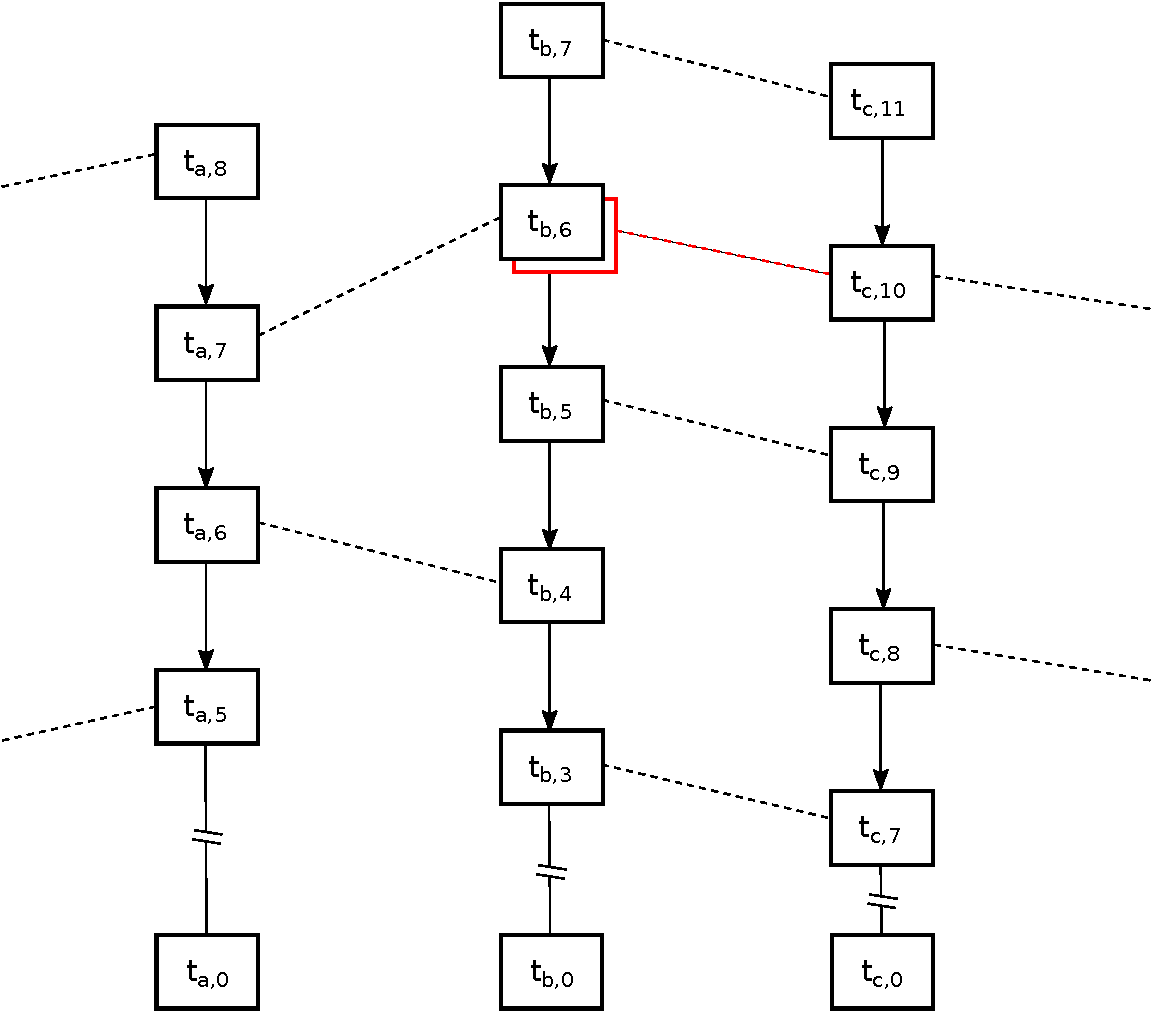
\includegraphics[width=0.9\textwidth]{trustchain-bad}
    \centering
    \caption{Every block is denoted by $t_{i,j}$, where $i$ is the node ID and $j$ is the sequence number of the block.
    Thus we have three nodes and three corresponding chains in this example.
    The arrows represent hash pointers and the dotted lines represent references.
    The blocks at the ends of one dotted line are pairs of each other.
    The red block after $t_{b, 5}$ indicate a fork.}
    \label{fig:trustchain-bad}
\end{figure}

If every node follows the rules of TrustChain and we only consider hash pointers,
then every chain effectively forms a singly linked list.
However, if a node violates the rules, then a \emph{fork} may happen.
That is, there may be more than one TX block with a hash pointer pointing back to the same block.
In \Cref{fig:trustchain-bad}, node $b$ (in the middle chain) created two TX blocks that both point to $t_{b, 5}$.
If this is a ledger system it can be seen as a double spend, where the currency accumulated up until $t_{b, 5}$ are spent twice.

\subsubsection*{Extended TrustChain}
We are now ready to explain the Extended TrustChain.
The primary difference is the introduction of a new type of block---checkpoint (CP) block.
In contract to TX blocks, CP blocks do not store transactions or contain references.
Their purpose is to capture the state of the chain and the state of the whole system.
In particular, the state of the chain is captured with a hash pointer.
The state of the whole system is captured in the content of the CP block,
namely as a digest of the latest \emph{consensus result} which we explain in \Cref{sec:overview-cons}.
A visual representation is shown in \Cref{fig:trustchain-bad-cp}.

From this point onwards, we use TrustChain to mean the Extended TrustChain unless explicitly clarified.

\begin{figure}
    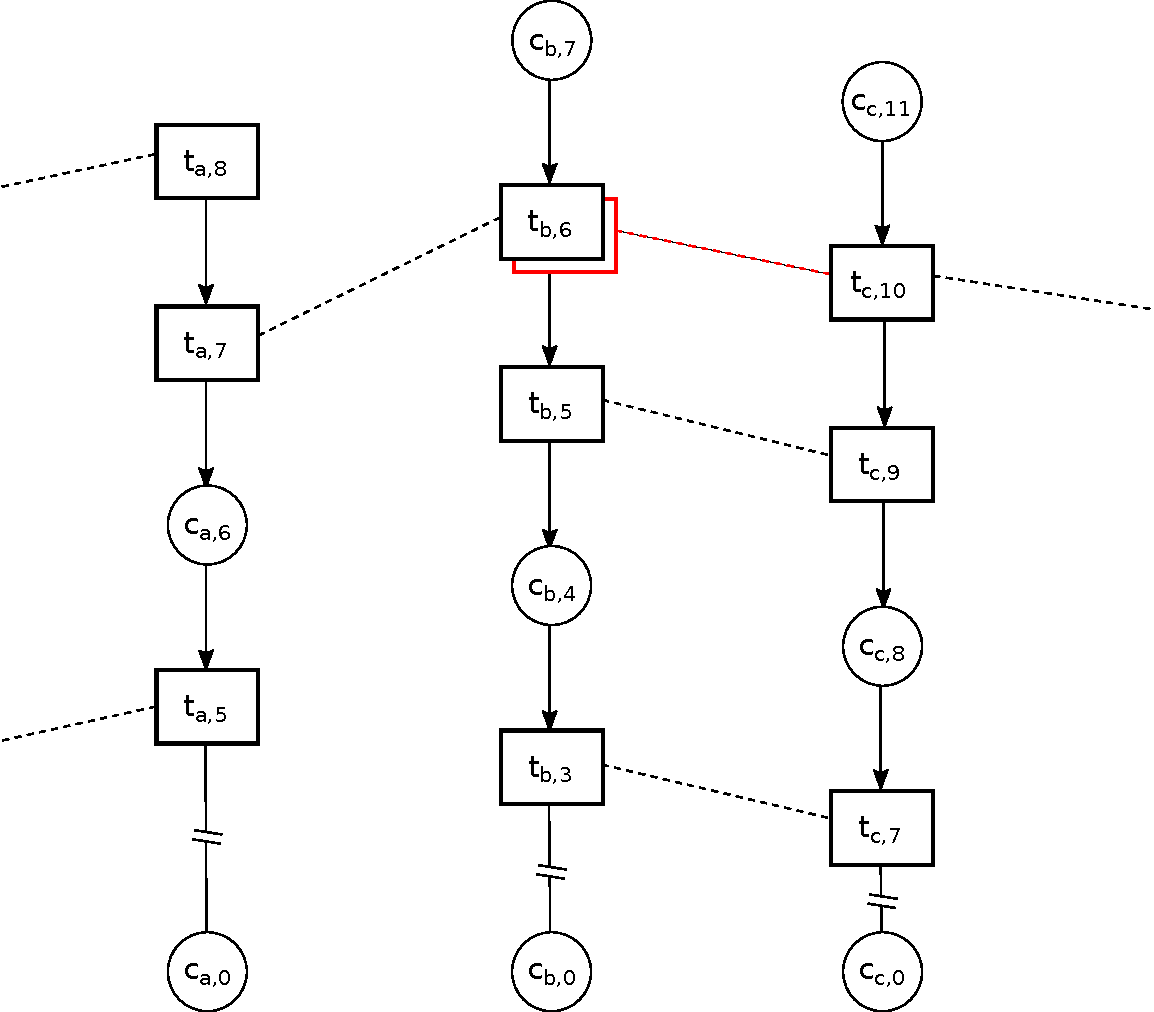
\includegraphics[width=0.9\textwidth]{trustchain-bad-cp}
    \centering
    \caption{The circles represent CP blocks,
    they also have hash pointers (arrow) but do not have references (dotted line).
    Note that the sequence number counter do not change, it is shared with TX blocks.}
    \label{fig:trustchain-bad-cp}
\end{figure}

\subsection{Consensus protocol}\label{sec:overview-cons}

% The consensus protocol uses an existing Byzantine consensus algorithm (explained in detail in \Cref{sec:xyz}) and runs it continuously in rounds.
The consensus protocol can be seen as a technique of running infinitly many rounds of some 
Byzantine consensus algorithm\footnote{More accuratly it is ACS or asynchronous subset consensus, we describe ACS in \Cref{sec:acs-background}.},
starting a new execution immediately after the previous one is completed.
This is necessary because blockchain systems always need to reach consensus on new values proposed by nodes in the system,
or CP blocks in our case.

The high communication complexity of Byzantine consensus algorithms prohibits us from running it on a large network.
Thus, for every round, we randomly select some node---called facilitators---to collect CP blocks from every other node and use them as the proposal.
The facilitators are elected using a \emph{luck value}, which is computed using $\textsf{H}(\C_r || pk_u)$,
where $\C_r$ is the consensus result 
(which can be seen as the set union of all the CP blocks collected by the facilitators)
in round $r$ and $pk_u$ is the public key of node $u$.
Intuitively, the election is guaranteed to be random 
because the output of a cryptographically secure hash function is unpredictable and $\C_r$ cannot be determined in advance.

A visual explaination can be found in \Cref{app:consensus-example},
it walks through the steps needed for a node to be selected as a facilitator using an example.

\subsection{Transaction and validation}
The TX protocol is a simple request and response protocol.
The nodes exchange one round of messages and create new TX blocks on their respective chains.
Thus, as we mentioned before, one transaction should result in two TX blocks.

The consensus and transaction protocol by themselves do not provide a mechanism to detect forks or other forms of tamperaing.
Thus we need a validation protocol to counteract malicious behaviour.
When a node wish to validate one of its TX, it asks the counterparty for the \emph{fragment} of the TX.
A fragment of a TX is a section of the chain beginning and ending with CP blocks that contains the TX and are in consensus.
Upon the counterparty's response, the node checks that the CP blocks are indeed in consensus,
the hash pointers are valid and his TX is actually in the fragment.
The TX is valid if these conditions are satisfied.
Intuitively, this works because it is hard (because a cryptographically secure hash function is second-preimage resistant)
to create a different chain that begins and ends with the same two CP blocks but with a different middle section.


\subsection{Combined protocol}
\label{sec:combined-protocol}
The final protocol is essentially the concurrent composition of the three aforementioned protocols,
all making use the Extended TrustChain data structure.

Our subprotocol design gives us the highly desireable non-blocking property.
In particular, we do not need to ``freeze'' the state of the chain for some communication to complete in order to create a block.
For instance, a node may start the consensus protocol, and while it is running, create new transactions and validate old transactions.
By the time the consensus protocol is done, the new CP block is added to whatever the state that the chain is in.
It is not necessary to lock the chain while the consensus protocol is running and then unlock it afterwards.

\section{Model and assumptions}
\label{sec:model-assumptions}

This section and the ones following it give a technical treatment of what the content in System Overview.
For notational clarity, we use the following convention (adapted from~\cite{miller2016honey}) throughout this work.
\begin{itemize}
\item Lower case (e.g. $x$) denotes a scalar object or a tuple.
\item Upper case (e.g. $X$) denotes a set or a constant.
\item Sans serif (e.g. $\textsf{fn}(\cdot)$) denotes a function.
\item Monospace (e.g. $\texttt{ack}$) denotes message type.
\end{itemize}
Further, we use $a || b$ to denote concatination of the binary representations of $a$ and $b$.

We assume purely asynchronous channels with eventual delivery.
Thus in no circumstance do we make timing assumptions.
The adversary has fully control of the delivery schedule and the message ordering of all messages.
But they are not allowed to drop messages except for their own\footnote{
    Reliability can be achieved in unreliable networks by resending messages or using some error correction code.
}.

We assume there exist a Public Key Infrastructure (PKI), and nodes are identified by their unique and permanent public key.
Finally, we use the random oracle model, i.e. calls to the random oracle are denoted by $\textsf{H}: \{0, 1\}^* \rightarrow \{0, 1\}^\lambda$,
where $\{0, 1\}^*$ denotes the space of finite binary strings and $\lambda$ is the security parameter~\cite{bellare1993random}.

In our model we consider $N$ nodes, which is the population size.
$n$ of them are facilitators, $t$ out of $n$ are malicious and the inequality
$n \ge 3t + 1$ must hold.
This is from the work of Pease, Shostak and Lamport, where they show a network of $n$ nodes cannot reach Byzantine agreement with $t \ge n/3$.
Further, the inequality $N \ge n + t$ must also hold.
This is due to our system design, which becomes clear in~\Cref{sec:consensus-phase}.

Our threat model is as follows. 
We use a restricted version of the adaptive corruption model.
The first restriction is that corrupted node can only change across rounds.
That is, if a round has started, the corrupted nodes cannot changed until the next round.
The second restriction is that the adversary, presumably controlling all the corrupted nodes, is forgetful.
Namely the adversary may learn the internal state such as the private key of a corrupted node,
but if the node recovers, then the adversary must forget the private key.
This is realistic because otherwise the adversary can eventually learn all the private keys and sabotage the system.
Finally, we assume computational security.
That is, the adversary can run polynomial-time algorithms but not exponential-time algorithms efficiently.

\section{Extended TrustChain}
The primary data structure used in our system is the Extended TrustChain.
Each node $u$ has a public and private key pair---$pk_u$ and $sk_u$, and a chain $B_u$.
The chain consist of blocks $B_u = \{ b_{u, i} : k \in \{ 0, \dots, h - 1 \} \}$,
where $b_{u, i}$ is the $i$th block of $u$,
and $h = |B_u|$.
We often use $b_{u, h}$ to denote the latest block.
There are two types of blocks, TX blocks and CP blocks.
If $T_u$ is the set of TX blocks of $u$ and $C_u$ is the set of CP blocks of $u$,
then it must be the case that $T_u \cup C_u = B_u$ and $T_u \cap C_u = \varnothing$.
The notation $b_{u, i}$ is generic over the block type.
We assume there exist a function $\textsf{typeof}: B_u \rightarrow \{ \tau, \gamma \}$ that returns the type of the block,
where $\tau$ represents the TX type and $\gamma$ represents the CP type.

\subsection{Transaction block}
The TX block is a six-tuple, i.e $t_{u, i} = \langle \textsf{H}(b_{u, i - 1}), seq_u, txid, pk_v, m, sig_u \rangle$.
We describe each item in turn.
\begin{enumerate}
\item $\textsf{H}(b_{u, i - 1})$ is the hash pointer to the previous block.
\item $seq_u$ is the sequence number which should equal $i$.
\item $txid$ is the transaction identifier, it should be generated using a cryptographically secure pseudo-random number generator by the initiator of the transaction.
\item $pk_v$ is the public key of the counterparty $v$.
\item $m$ is the transaction message.
\item $sig_u$ is the signature created using $sk_u$ on the concatination of the binary representation of the five items above.
\end{enumerate}
The fact that we have no constraint on the content of $m$ is in alignment with our design goal---application neutrality.

TX blocks come in pairs.
In particular, for every block 
$$t_{u, i} = \langle \textsf{H}(b_{u, i - 1}), seq_u, txid, pk_v, m, sig_u \rangle$$
there exist one and only one \emph{pair} 
$$t_{v, j} = \langle \textsf{H}(b_{v, j - 1}), seq_v, txid, pk_u, m, sig_v \rangle.$$
Note that the $txid$ and $m$ are the same, and the public keys refer to each other.
Thus, given a TX block, these properties allow us to identify its pair.

% TODO Node $v$ may cheat and create more than one pair for $t_{u, i}. we discuss later

\subsection{Checkpoint block}

The CP block is a five-tuple, 
i.e. $c_{u, i} = \langle \textsf{H}(b_{u, i-1}), seq_u, \textsf{H}(\C_r), r, sig_u \rangle$,
where $\C_r$ is the consensus result (which we describe in \Cref{sec:consensus-result}) in round $r$, the other items are the same as the TX block definition.
Note that unlike in our prior work~\cite{implicitconsensus}, CP blocks and TX blocks do not have independent sequence numbers.

The genesis block in the chain must be a CP block in the form of
$c_{u, 0} = \langle \textsf{H}(\bot), 0,  \textsf{H}(\bot), 0, sig_u \rangle$
where $\textsf{H}(\bot)$ can be interpreted as applying the hash function on an empty string.
The genesis block is unique because every node has a unique public and private key pair.


\subsection{Consensus result}
\label{sec:consensus-result}
Our consensus protocol runs in rounds as discussed in \Cref{sec:system-overview}.
Every round is identified by a round number $r$, which is incremented on every new round.
The consensus result is a tuple, i.e. $\C_r = \langle r, C \rangle$,
where $C$ is a set of CP blocks agreed by the facilitators of round $r$.

\subsection{Chain properties}
Here we define a few important properties which results from the interleaving nature of CP and TX blocks.

If there exist a tuple $\langle c_{u,a}, c_{u, b} \rangle$ for a TX block $t_{u, i}$,
where 
$$a = \argmin_{k, k < i, \texttt{typeof}(b_{u,k}) = \gamma}(i - k)$$
$$b = \argmin_{k, k > i, \texttt{typeof}(b_{u,k}) = \gamma}(k - i),$$
then $\langle c_{u,a}, c_{u, b} \rangle$ is the \emph{enclosure} of $t_{u, i}$.
Note that $c_{u, a}$ is the more recent CP block.
Also, some TX blocks may not have any subsequent CP blocks, then its enclosure is $\bot$.

If the enclosure of some TX block $t_{u, i}$ is $\langle c_{u,a}, c_{u, b} \rangle$,
then its \emph{fragment} $F_{u, i}$ is defined as $\{ b_{u, i} : a \le i \le b \}$.
For convenience, the function $\textsf{fragment}(\cdot)$ represents the fragment of some TX block if it exists, otherwise $\bot$.

\emph{Agreed enclosure} is the same as enclosure with an extra constraint where the CP blocks must be in some consensus result $\C_r$ and also must be the smallest enclosure.
That is, suppose a chain is in the form
    $\{c_{i}, c_{i+1}, t_{i+2}, c_{i+3}\}$\footnote{Usually the notation is of the form $c_{u, i}$, but the node identity is not important here so we simplify it to $c_{i}$}
    and $c_{i}, c_{i+1}, c_{i+3}$ are in $\C_r, \C_{r+1}, \C_{r+3}$ respectively,
    then the agreed enclosure of $t_{i+2}$ is $\langle c_{i+1}, c_{i+3}\rangle$ and cannot be $\langle c_{i}, c_{i+3}\rangle$.
Similarly, \emph{agreed fragment} has the same definition as fragment but using agreed enclosure.
We define its function to be $\textsf{agreed\_fragment}(\cdot)$ which we use later in the validation protocol (\Cref{sec:vd-protocol}).

% The length of the fragment is constrained by $L$,
% namely $\forall t |\textsf{fragment}(t)| \le L$.
% The purpose to prevent spam and encourage nodes to create more CP blocks.
% $L$ should be sufficiently high so that busy nodes are not hindered by it.


\section{Consensus protocol}
\label{sec:cons-protocol}

Our consensus protocol runs on top of Extended TrustChain.
It is directly related to the creation of CP blocks.
The objectives of the protocol are to
    allow honest nodes always make progress (in the form of creating new CP blocks),
    compute correct consensus result in every round
    and have unbiased election of facilitators.
Concretely, we define the necessary properties as follows.
\begin{definition}
\label{def:consensus}
\textbf{\emph{Properties of the consensus protocol}}

$\forall r \in \mathbb{N}$, the following properties must hold.
\begin{enumerate}
    \item \emph{Agreement}:
        If one correct node outputs a set of facilitators $\F_r$,
        then every node outputs $\F_r$
    \item \emph{Validity}:
        If any correct node outputs $\F_r$, then 
            \begin{enumerate}
                \item $|\C_r| \ge N - t$ must hold for the $\C_r$ which was used to create $\F_r$,
                \item $\F_r$ must contain at least $n - t$ honest nodes and
                \item $|\F_r| = n$.
            \end{enumerate}
    \item \emph{Fairness}:
        Every node with a CP block in $\C_r$ should have an equal probability of becoming a member of $\F_r$.
    \item \emph{Termination}:
        Every correct node eventually outputs some $\F_r$.
\end{enumerate}
\end{definition}
These properties may look like Byzantine consensus properties (which we describe next in \Cref{sec:acs-background}) but they have some subtle differences.
Firstly, they are properties for every node in the network and not just the facilitators.
Secondly, they must be satisfied for all rounds because the whole system falls apart if one of the property cannot be satisfied in one of the rounds.

Before describing the protocol in detail,
we take a brief detour to give background on the asynchronous subset consensus.
This is the primary building block of our protocol.
% Starting with the bootstrap phase and then moving on to the actual consensus phase.

\subsection{Background on asynchronous subset consensus}
\label{sec:acs-background}

The best way to explain asynchronous subset consensus (ACS) is to contrast it with the typical Byzantine consensus.
We adapt the description from~\cite[Chapter 17]{podc}.
%The Byzantine consensus problem is a classical problem is distributed systems literature.
%It is first described by Leslie Lamport as the Byzantine general's problem in 1982~\cite{lamport1982byzantine}.
%Byzantine consensus is described as follows (adapted from ).
\begin{definition}
\textbf{\emph{Byzantine Consensus}}

There are $n$ nodes, of which at most $t$ might experience Byzantine fault.
Node $i$ starts with an input value $v_i$.
The nodes must decide for one of  those values, satisfying the the following.
\begin{enumerate}
    \item \emph{Agreement:}
        If a correct node outputs $v$, then every node outputs $v$.
    \item \emph{Validity:}
        The decision value must be the input value of a node.
    \item \emph{Termination:}
        All correct nodes terminate in finite time.
\end{enumerate}
\end{definition}
A node under Byzantine fault means that it can have arbitrary behaviour.
For example not sending message or colluding with other Byzantine nodes to undermine the entire system.
Note that the decision is on a single value.
This is in contrast to ACS which we describe next.

ACS shares many similarities with Byzantine consensus.
But it is an especially useful primitive for blockchain systems.
It allows any party to propose a value and the result is the set union of all the proposed values by the majority.
This is the primary difference with Byzantine consensus.
Concretely, ACS needs to satisfy the following properties (adapted from~\cite{miller2016honey}).
\begin{definition}
\label{def:acs}
\textbf{\emph{Asynchronous Subset Consensus}}

There are $n$ nodes, of which at most $t$ might experience Byzantine fault.
Node $i$ starts with an non-empty set of input values $C_i$.
The nodes must decide an output $C$, satisfying the following.
\begin{enumerate}
    \item \emph{Agreement:}
        If a correct node outputs $C$, then every node outputs $C$.
    \item \emph{Validity:}
        If any correct node outputs a set $C$,
        then $|C| \ge n - t$ and $C$ contains the input of at least $n - 2t$ nodes.
    \item \emph{Totality:}
        If $n - t$ nodes receive an input, then all correct nodes produce an output.
\end{enumerate}
\end{definition}

ACS has the nice property of censorship resiliance when compared to other consensus algorithms.
For instance, Hyperledger and Tendermint uses Practical Byzantine Fault Tolerance (PBFT)~\cite{castro1999practical} as their consensus algorithm.
In PBFT, a leader is elected, if the leader is malicious but follows the protocol, then it can selectivly filter transactions.
In contract, every party in ACS are involved in the proposal phase,
and it guarantees that if $n - 2t$ parties propose the same transaction, then it must be in the agreed output.
Thus, if some value is submitted to at least $n - 2t$ nodes, it is guaranteed to be in the consensus result.
For a detailed description of ACS we refer to the HoneyBadgerBFT work~\cite{miller2016honey}.

The main drawback with ACS and also Byzantine consensus algorithms is the high message complexity.
Typically, such protocols have a message complexity of $O(n^2)$, where $n$ is the number of parties.
Hence, it may work with a small number of nodes,
but it is infeasible for blockchain systems where thousands of nodes are involved.

% The literature on Byzantine consensus and atomic broadcast is rich, some noteable ones include TODO.
% Thus in the ETC consensus protocol, we assume there exist an "off-the-shelf" Byzantine consensus algorithm which we can use
% (in our implementation we use HoneyBadgerBFT and motivate our choice in TODO).

% In our case, every node do not propose some arbitrary data, but a set of CP blocks.
% Thus the result of the consensus is the set union of all the legitimate proposals.


\subsection{Bootstrap phase}
\label{sec:bootstrap}
Now we have all the necessary information to describe our consensus protocol.
We begin with the bootstrap phase and then move onto the actual consensus phase.

Recall that facilitators are computed from the consensus result,
but the consensus result is agreed by the facilitators.
Thus we have a dependency cycle.
The goal of the bootstrap phase is to give us a starting point in the cycle.

To bootstrap, imagine that there is some bootstrap oracle, that initiates the code on every node.
The code satisfied all the properties in \Cref{def:consensus}.
Namely every node has the same set of valid facilitators $\F_1$ that are randomly choosen.
This concludes the bootstrap phase.

In practice, the bootstrap oracle is most likely the software developer and some of the desired properties cannot be achieved.
In particular, it is not possible to have the fairness property because it is unlikely that the developer knows the identity of every node in advance.

\subsection{Consensus phase}
\label{sec:consensus-phase}
The consensus phase begins when $\F_r$ is available to all the nodes.
Note that $\F_r$ indicates the facilitators that were elected using result of round $r$ and are responsible for driving the ACS protocol in round $r + 1$.
The goal is to reach agreement on a set of new facilitators $\F_{r + 1}$ that satisfies the four properties in \Cref{def:consensus}.

There are two scenarios in the consensus phase.
First, if node $u$ is not the facilitator, it sends $\langle \texttt{cp\_msg}, c_{u, h} \rangle$ to all the facilitators.
Second, if the node is a facilitator, it waits until it has received $N - t$ messages of type \texttt{cp\_msg}.
% Second if the node is a facilitator, it waits for some duration $D$ and collect messages of type \texttt{cp\_msg}, where $D \gg \Delta$.
Invalid messages are removed, namely blocks with invalid signatures and duplicate blocks signed by the same key.
With the sufficient number of \texttt{cp\_msg} messages,
it begins the ACS algorithm and some $\C'_{r + 1}$ should be agreed upon by the end of it.
Duplicates and blocks with invalid signatures are again removed from $\C'_{r+1}$ and we call the final result $\C_{r+1}$
We have the remove invalid blocks a second time (after ACS) because the adversary may send different CP blocks to different facilitators,
which results in invalid blocks in the ACS output.

At the core of the consensus phase is the ACS protocol.
While any ACS protocol that satisfies the standard definition will work,
we use a simplification of HoneyBadgerBFT~\cite{miller2016honey} as our ACS protocol
because it is the only (to the best of our knowledge) consensus algorithms designed for blockchain systems.
We do not use the full HoneyBadgerBFT due to the following.
First, the transactions in HoneyBadgerBFT are first queued in a buffer and the main consensus algorithm starts only when the buffer reaches an optimal size.
We do not have an infinite stream of CP blocks, thus buffering is unsuitable.
Second, HoneyBadgerBFT uses threshold encryption to hide the content of the transactions.
But we do not reach consensus on transactions, only CP blocks, so hiding CP blocks is meaningless for us as it contains no transactional information.

Continuing, when $\F_{r}$ reaches agreement on $\C_{r+1}$,
they immediately broadcast two messages to all the nodes---
first the consensus message $\langle \texttt{cons\_msg}, \C_{r+1} \rangle$,
and second the signature message $\langle \texttt{cons\_sig}, r, sig \rangle$.
The reason for sending \texttt{cons\_sig} is the following.
Recall that channels are not authenticated, 
and there are no signatures in $\C_{r + 1}$.
If a non-facilitator sees some $\C_{r + 1}$, it cannot immediately trust it because it may have been forged.
Thus, To guarantee authenticity, every facilitator sends an additional message that is the signature of $\C_{r + 1}$.

Upon receiving $\C_{r + 1}$ and at least $n - f$ valid signatures by some node $u$, $u$ performs two asks.
First, it creates a new CP block using $\textsf{new\_cp}(\C_{r + 1}, r + 1)$ (\Cref{alg:new-cp}).
Second, it computes the new facilitators using $\textsf{get\_facilitator}(C, n)$ (\Cref{alg:facilitator})
and updates its facilitator set to the result.
This concludes the consensus phase and brings us back to the beginning of the consensus phase.

\begin{algorithm}
\caption{Function $\textsf{get\_facilitator}(C, n)$ takes a set of CP blocks $C$ and an integer $n$,
sort evey element in $C$ by its luck value (the $\lambda$-expression), and outputs the smallest $n$ elements.}
\label{alg:facilitator}
\begin{algorithmic}
\State $\textsf{take} (n, \textsf{sort\_by} (\lambda x.\textsf{H}(x || pk \text{ of } x), C))$
\end{algorithmic}
\end{algorithm}

\begin{algorithm}
\caption{Function $\textsf{new\_cp}(\C_r, r)$ runs in the context of the caller $u$.
It creates a new CP block and appends it to $u$'s chain.}
\label{alg:new-cp}
\begin{algorithmic}
\State $h \gets |B_u|$
\State $c_{u, h} \gets \langle \textsf{H}(b_{u, h-1}), h, \textsf{H}(\C_r), r, sig_u \rangle$
\State $B_u \gets B_u \cup c_{u, h}$
\end{algorithmic}
\end{algorithm}

Our protocol has some similarities with synchronisers~\cite[Chapter 10]{podc} because it is effectively a technique to introduce synchrony in an asynchronous environment.
If we consider the facilitators is a collective authority, then it can be seen as a synchroniser that sends pulse messages (in the form of \texttt{cons\_msg} and \texttt{cons\_sig}) to indicate the start of a new clock pulse.
Every node then sends a completion messages (in the form of \texttt{cp\_msg}) to the collective authority to indicate that they are ready to start a new pulse.


\section{Transaction protocol}
\label{sec:tx-protocol}

The TX protocol, shown in \Cref{alg:tx-proto}, is run by all nodes.
It is also known as True Halves, first described by Veldhuisen~\cite[Chapter~3.2]{truehalves}.
Node that wish to initiate a transaction calls $\textsf{new\_tx}(pk_v, m, txid)$ (\Cref{alg:new-tx}) with the intended counterparty $v$ identified by $pk_v$ and message $m$.
$txid$ should be a uniformly distributed random value, i.e. $txid \in_R \{0, 1\}^{256}$.
Then the initiator sends $\langle \texttt{tx\_req}, t_{u, h}\rangle$ to $v$.

\begin{algorithm}
    \caption{Function $\textsf{new\_tx}(pk_v, m, txid)$ generates a new TX block and appends it to the caller $u$'s chain.
    It is executed in the private context of $u$, i.e. it has access to the $sk_u$ and $B_u$.
    The necessary arguments are the public key of the counterparty $pk_v$, the transaction message $m$ and the transaction identifier $txid$.}
    \label{alg:new-tx}

    \begin{algorithmic}
    \State $h \gets |B_u|$
    \State $t_{u, h} \gets \langle \textsf{H}(b_{u, h - 1}), h, txid, pk_v, m, sig_u \rangle$
    \State $B_u \gets B_u \cup \{ t_{u, h} \}$
    \end{algorithmic}
\end{algorithm}

\begin{algorithm}
    \caption{The TX protocol which runs in the context of node $u$.}
    \label{alg:tx-proto}

    \begin{algorithmic}
        \Upon $\langle \texttt{tx\_req}, t_{v, j} \rangle$ from $v$
        \State $\langle \_, \_, txid, pk_v, m, \_ \rangle \gets t_{v, j}$
        \State $\textsf{new\_tx}(pk_u, m, txid)$
        \State store $t_{v, j}$ as the pair of $t_{u, h}$
        \State send $\langle \texttt{tx\_resp}, t_{u, h} \rangle$ to $v$

        \Upon $\langle \texttt{tx\_resp}, t_{v, j} \rangle$ from $v$
        \State $\langle \_, \_, txid, pk_v, m, \_ \rangle \gets t_{v, j}$
        \State store $t_{v, j}$ as the pair of the TX with identifier $txid$
    \end{algorithmic}
\end{algorithm}

A key feature of the TX protocol is that it is non-blocking.
At no time in \Cref{alg:new-tx} or \Cref{alg:tx-proto} do we need to hold the chain state and wait for some message to be delivered before committing a new block to the chain.
This allows for high concurrency where we can call $\textsf{new\_tx}(\cdot)$ multiple times without waiting for the corresponding \texttt{tx\_resp} messages.

\section{Validation protocol}
\label{sec:vd-protocol}

Up to this point, we do not provide a mechanism to detect forks or other forms of tampering or forging.
The validation protocol aims to solve this issue.
The protocol is also a request-response protocol, just like the transaction protocol.
But before explaining the protocol itself, we first define what it means for a transaction to be valid.

\subsection{Validity definition}
A transaction can be in one of three states in terms of validity---\emph{valid}, \emph{invalid} and \emph{unknown}.
Given a fragment $F_{v, j}$, the validity of the transaction $t_{u, i}$ is captured by the function $\textsf{get\_validity}(t, F)$ (\Cref{alg:get-validity}).
The first four conditions (up to \Cref{line:valid-fragment}) essentially check whether the fragment is the one that the verifier needs.
If it is not, then the verifier cannot make any decision and return \emph{unknown}.
This is likely to be the case for new transactions because $\textsf{agreed\_fragment}(\cdot)$ would be $\bot$.
The next two conditions checks for tampering or missing blocks, if any of these misconducts are detected, then the TX is invalid.

Note that the validity is on a transaction (two TX blocks with the same $txid$), rather than on one TX block owned by a single party.
It is defined this way because the malicious sender may create new TX blocks in their own chain but never send \texttt{tx\_req} messages.
In that case, it may seem that the counterparty, who is honest, purposefully ommitted TX blocks.
But in reality, it was the malicious sender who did not follow the protocol.
Thus, in such cases the whole transaction, identified by its $txid$ is marked as invalid.

Further, the caller of $\textsf{get\_validity}(t_u{u, i}, F_{v, i})$ is not necessarily 
$u$\footnote{In practice it often is because after completing the TX protocol the parties are incentivised to check that the counterparty ``did the right thing''.}
Any node $w$ may call $\textsf{get\_validity}(t_u{u, i}, F_{v, i})$ as long as the caller $w$ has an agreed fragment of $t_{u, i}$---$F_{u, i}$.
$F_{u, i}$ may be readily available if $w = u$ or it may be from some other \texttt{vd\_resp} message, which we describe next in the validation protocol.

\begin{algorithm}
\caption{Function $\textsf{get\_validity}(t_{u, i}, F_{v, j})$ validates the transaction $t_{u, i}$.
$F_{v, j}$ is the corresponding fragment received from $v$.}
We assume there exist a valid $F_{u, i}$, namely the agreed fragment of $t_{u, i}$. 
The caller is $w$, it may be $u$ but this is not necessary.
\label{alg:get-validity}

\begin{algorithmic}[1]

    % \State $F_{u, i} \gets \textsf{agreed\_fragment}(t_{u, i})$
    % \If{$F_{u, i} = \bot$}
    %     \State \Return \emph{unknown}
    % \EndIf \Comment $u$ has agreed fragment
    % \State 

    \State $c_{v, a} \gets \textsf{first}(F_{v, j})$
    \State $c_{v, b} \gets \textsf{last}(F_{v, j})$
    \If{$c_{v, a}$ or $c_{v, b}$ are not in consensus}
        \State \Return \emph{unknown}
    \EndIf
    \State \Comment $v$ has agreed fragment

    % \If{$|F_{v, j}| > L$}
    %     \State \Return \emph{unknown}
    % \EndIf \Comment fragment not too long
    % \State

    % txid are equal now, but bad hash pointer
    \If{sequence number in $F_{v, j}$ is correct (sequential)}
        \If{hash pointers in $F_{v, j}$ is wrong}
            \State \Return \emph{unknown}
        \EndIf
    \EndIf
    \State \Comment correct TrustChain structure

    \State $c_{u, b} \gets \textsf{last}(F_{u, i})$
    \If{$c_{u, b}$ is not created using the same $\C_r$ as $c_{v, b}$}
        \State \Return \emph{unknown}
    \EndIf
    \State \Comment correct consensus round
    \label{line:valid-fragment}
    \State $\langle \_, \_, txid, pk_v, m, \_ \rangle \gets t_{u, i}$
    \If{number of blocks of $txid$ in $F_{v, j} \ne 1$}
        \State \Return \emph{invalid}
    \EndIf
    \State \Comment TX exists 

    \State $\langle \_, \_, txid', pk'_u, m', \_ \rangle \gets t_{v, j}$
    \If{$m \ne m' \vee pk_u \ne pk'_u$}
        \State \Return \emph{invalid}
    \EndIf
    \State \Comment no tampering
    \State \Return \emph{valid}
\end{algorithmic}
\end{algorithm}

\subsection{Validation protocol}
With the validity definition, we are ready to construct a protocol for determining the validity of transactions.
The protocol is a simple response and request protocol (\Cref{alg:vd-proto}).
If $u$ wishes to validate some TX with ID $txid$ and counterparty $v$, it sends $\langle \texttt{vd\_req}, txid \rangle$ to $v$.
The desired properties of the validation protocol are as follows.
\begin{definition}
\label{def:validation}
\textbf{\emph{Properties of the validation protocol}}

\begin{enumerate}
    \item \emph{Agreement}:
        If any correct node decides on the validity (except when it is \emph{unknown}) of a transaction,
        then all other correct nodes are able to reach the same conclusion or \emph{unknown}.
    \item \emph{Correctness}:
        The validation protocol outputs the correct result
        according to the aforementioned validity definition.
    % \item \emph{Unforgeability}:
    %     If some transaction is valid, it cannot be forged into an invalid transaction.
    %     If some transaction is invalid, it cannot be forged into a valid transaction.
    \item \emph{Liveness}:
        Any valid (invalid) transactions is marked as valid (invalid) eventually.
\end{enumerate}
\end{definition}

\begin{algorithm}
\caption{Validation protocol}
\label{alg:vd-proto}

\begin{algorithmic}
    \Upon $\langle \texttt{vd\_req}, txid \rangle$ from $v$
        \State $t_{u, i} \gets \text{the transaction identified by } txid$
        \State $F_{u, i} \gets \textsf{agreed\_fragment}(t_{u, i})$
        \State send $\langle \texttt{vd\_resp}, txid, F_{u, i} \rangle$ to $v$

    \Upon $\langle \texttt{vd\_resp}, txid, F_{v, j} \rangle$ from $v$
        \State $t_{u, i} \gets \text{the transaction identified by } txid$
        \State set the validity of $t_{u, i}$ to $\textsf{get\_validity}(t_{u, i}, F_{v, j})$
\end{algorithmic}
\end{algorithm}

We make two remarks.
First, just like the TX protocol, we do not block at any part of the protocol.
Second, suppose some $F_{v, j}$ validates $t_{u, i}$, then that does not imply that $t_{u, i}$ only has one pair $t_{v, j}$.
Our validity requirement only requires that there is only one $t_{v, j}$ in the correct consensus round.
The counterparty may create any number of fake pairs in a later consensus rounds.
But these fake pairs only pollutes the chain of $v$ and can never be validated because the round is incorrect.

\section{Design variations and tradeoffs}
\label{sec:tradeoffs}

Up to this point,
we have discussed our protocol in the context of the model and assumptions defined in \Cref{sec:model-assumptions}.
In this section, 
we explore a few design variations which we can make, some of them require a relaxed version of our original model.
They enable better performance, allow us to apply our design in the fully permissionless setting and improves privacy.

\subsection{Using epidemic protocol to reduce communication cost}
One of the final steps in our consensus protocol is to broadcast the consensus result and signatures to every other node (\Cref{sec:consensus-phase}).
While this guarantees delivery (since we assumed reliable channel), it is wasteful.
For example, if every facilitator is honest, a node would receive $n$ consensus results which are identical when only one is necessary.

An optimisation we can do is to use an epidemic protocol~\cite{eugster2004epidemic} (also known as gossiping)) instead of our broadcast approach.
Typical epidemic protocols works as follows.
Every node buffers every message it receives up to some buffer size $b$.
Then it forwards the messages $t$ number of times.
Every time the message is sent to $f$ random neighbours, $f$ is often called the fan-out.
The upside of using epidemic protocol is that the communication cost is distributed more evenly between nodes.
This is especially true with a lazy push approach the node who just received a message would push the message ID to its $f$ random neighbours,
and only push the full message if the neighbour explicitly requests for the message~\cite{leitao2007epidemic}.
With this, nodes typically only need to receive one consensus result message instead of $n$.

A down side of epidemic protocol is that it usually takes $O(\log N)$ time to infect the whole network,
whereas broadcasting uses constant time.
Another downside of some epidemic protocols (e.g. eager push) is that it is difficult to guarantee delivery.
It is especially true when the parameters are not choosen correctly in a network that is only partially connected (but every node is nevertheless reachable).
If the delivery cannot be guaranteed, 
then we cannot guarantee liveness in our consensus protocol because a future facilitator may miss the memo.
Picking parameters are difficult in practice because the network configuration is unknown and the total number of nodes might also be unknown.


\subsection{Using timing assumption in the permissionless setting}
Our model is purely asynchronous, where we make no timing assumptions anywhere in the protocol.
In many applications however, it is often fine to make timing assumptions.
For example, TCP relies on timeout for its retransmission and the nLockTime property in Bitcoin transactions makes the transaction unspendable until some time in the future (either Unix time or block height)~\cite{bitcoindevguide}.
One limitation of our system is that we use the parameter $N$ in our algorithms, which makes it unsuitable for the permissionless environment where users can join and leave at will.
In this section we show how making a timing assumption would allow us to operate in the permissionless setting.

At the start of our consensus phase (\Cref{sec:consensus-phase}), facilitators must wait for $N-f$ \texttt{cp\_msg} messages.
This is the only place where we used $N$ as a parameter.
To introduce timing, instead of waiting for $N-f$ messages, we wait for some time $D$,
such that $D$ is sufficiently long for honest nodes to send their CP blocks to the facilitators.
Again, choosing the parameter $D$ is difficult and depends on a number of factors such as the network condition, message size, and so on.
Overestimating it would make agreed fragments much longer than usual, which increases communication costs for validation.
Underestimating it would lead to unfairness where users that are too late do not have a chance to be selected as a facilitator in the next round.
Nevertheless, there is a significant gain for making the timing assumption and that is the ability to operate in the permissionless setting which we explain next.

Suppose a new node wish to join the network and the facilitators are known (this can be done with a public registry).
It simply sends its latest CP block to the facilitators.
Then, in the next round the node will have a chance to become a facilitator just like any existing node.
To leave the network, nodes simply stop submitting CP blocks.
There is a subtlety here which happens when the node is elected as a facilitator in the following round.
In this case, the node must fulfill its oblication by completing the consensus protocol (but without proposing its own CP block) before leaving.
Otherwise the $n \ge 3t + 1$ condition may be violated.

\subsection{Privacy preserving validation protocol using compact blocks}
\label{sec:compact}
Our approach already has privacy preserving features in comparison to early blockchain systems.
That is, the transactions for each node are only revealed during the validation protocol.
Hence if two nodes never directly or indirectly interact with each other,
their transactions are never revealed.

We can take our privacy-preserving property one step further by introducing another level of hash pointer indirection.
The result is shown in~\Cref{fig:compact}.
\begin{figure}
    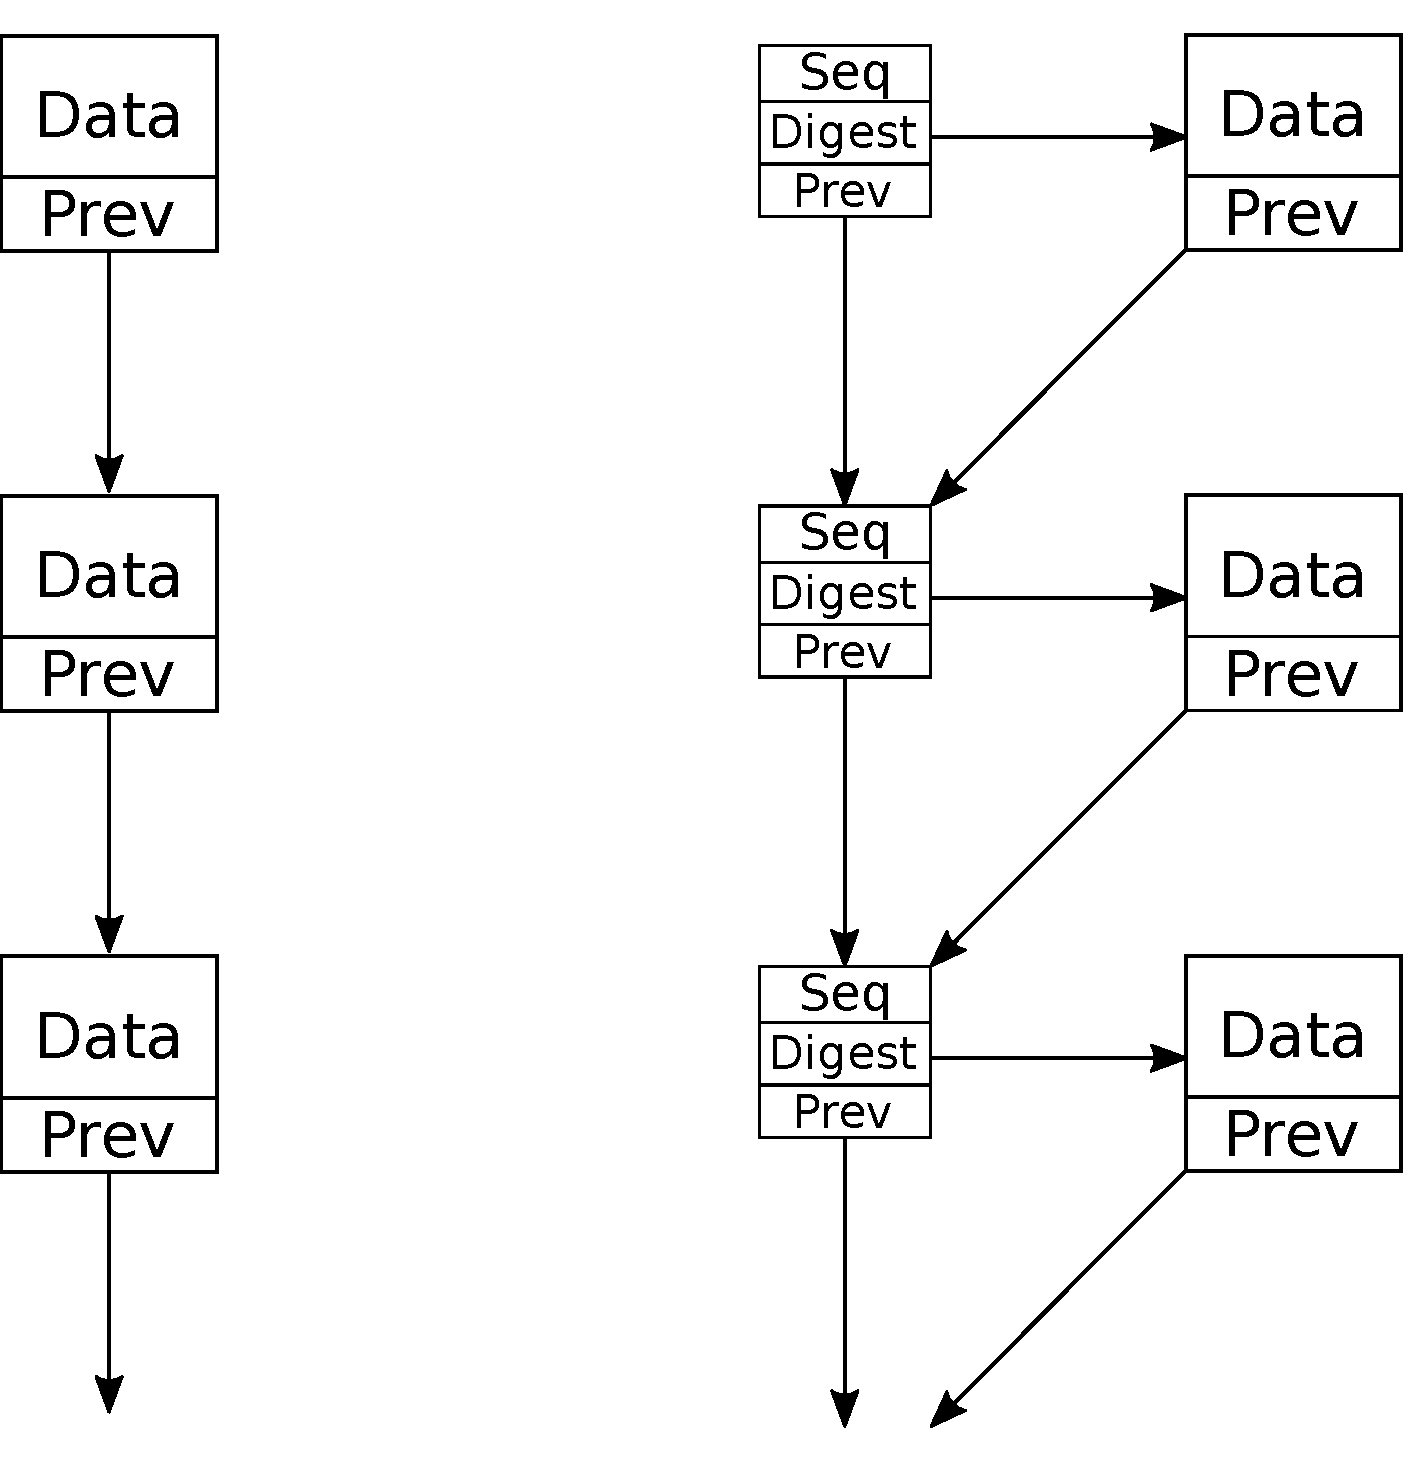
\includegraphics[width=0.7\textwidth]{compact}
    \centering
    \caption{The chain on the left represent direct chaining, where the digest in ``Prev'' is simply the digest of the previous block.
    The chain on the right uses compact blocks, represented by the smaller squares.
    Compact blocks also form a chain as before, but they each have a hash pointer to the full block, identified by ``Seq'' or ``Digest''.}
    \label{fig:compact}
\end{figure}

Concretely, we introduce an additional block type,
namely compact block.
Such blocks only have three attributes,
\begin{enumerate}
\item Seq---the sequence number its corresponding block,
\item Digest---the digest of its corresponding block, and
\item Prev---the digest of the previous compact block.
\end{enumerate}
Each compact block has a corresponding full block (either a CP block or a TX block).
The relationship is uniquely identified with Seq or Digest.
Recall that our original validation protocol requires the nodes to send the full agreed fragment.
With compact blocks, it is only necessary to send the compact version of the agreed fragment.
The validation then proceeds in a similar fashion,
provided that the pair of the to-be-validated TX block is known.

The space saving of this approach of course depends on the size of the full blocks.
If the full blocks are on average 500 bytes
(which is the typical size of Bitcoin transactions ~\cite{txsize}),
and the compact blocks are $32 + 32 + 8 = 72$ bytes
(SHA256 digests are 32 bytes each and we use a 64 bit integer to represent the sequence number),
then we have a 86\% saving in communication cost.

%Using compact blocks, it is possible to reduce network communication costs in the validation protocol but also protect transaction privacy.

\subsection{Optimising validation protocol using cached agreed fragments}
\label{sec:caching}
One more way to improve the efficiency of the validation protocol is to use a single agreed fragment to validate multiple transaction.
Concretely, upon receiving an agreed fragment from node $A$,
rather than validating a single transaction,
we attempt to validate all transactions in the unknown state performed with $A$ in that fragment.

For a node, the benefit of this technique is maximised when it only transacts with one other node.
In this case, the communication of one fragment is sufficient to validate all transactions in that fragment.
In the opposite extreme, if every transaction that the node makes is with another unique node,
then the caching mechanism would have no effect.

\subsection{Global fork detection}
The validation algorithm guarantees that there are no forks within a single agreed fragment.
This is sufficient for some applications such as proving the existance of some information.
However, applications such as digital cash where every block depends on some previous block,
then our scheme is not suitable.

There are a variety of approaches to do global fork detection.
First and the easiest solution is to simply ask for every agreed fragment from the one containing the genesis block up to the one that the to-be-proven TX block is in.
If the hash pointers are correct and all the CP blocks are in consensus, then the verifier can be sure that there are no forks.
We use this approach in our prior work on Implicit Consensus~\cite{implicitconsensus}.
It may sound inefficient at first, but nodes can employ caching to minimise communication costs.
In our work we call this ``spontaneous sharding''.

The second approach is probabilistic but with only a constant communication overhead.
For a node, observe that if every of its agreed fragment has a transaction with a honest node,
then the complete chain is effectively validated in a distributed maner.
The only way for an attacker to make a fork is to make sure that the agreed fragment containing the fork has no transactions with honest nodes.
We claim such malicious behaviour is prevented probabilisticaly using a challenge-response protocol as follows.
Suppose node $A$ wish to make a transaction with node $B$.
$A$ first sends a challenge to $B$ asking it to proof that it holds a valid agreed fragment between some consensus round specified by $A$.
If $B$ provides a correct proof, then they run the transaction protocol as usual.
If $B$ provides an invalid proof or refuses to respond,
then $A$ would refuse to make the transaction.
The probability that an honest node catches out a malicious node is 
$$p = \frac{f}{r},$$
where $f$ is the number of bad agreed fragments and $r$ is the latest round number.
If there are more nodes (say $n$) trying to make transactions with the malicious node,
then the probability that the malicious node does gets caught at least once follows a binomial distribution
$$\Pr[X > 0] = \sum_{k = 1}^{n}\binom{n}{k}p^k (1 - p)^{n - k}.$$

% subtlety when fork happens on CP block


% Another assumption we made in this work is the existance of a PKI.
% This can also be removed with the introduction of timing by storing the public keys the consensus results,
% much like in Bitcoin.


% \section{Universally Composable Framework}
% \label{sec:uc-intro}

% In order to analyse the security of a system, a formal notion of security is required.
% For instance, what does it mean if an encryption algorithm is secure?
% One may say it is secure if the adversay cannot learn any information about the plaintext from the ciphertext.
% But what if the adversay has some background information, for instance she may know it is English.
% Do we then still say the encryption algorithm is secure?
% Goldwasser and Micali introduced the notion of semantic security~\cite{goldwasser1982probabilistic}.
% That is, imagine two worlds, a real world and an ideal world.
% In the real world, the adversay is given the ciphertext,
% and in the ideal world the adversay has nothing.
% Then the encryption algorithm is semantically secure if the amount of information that the adversay can learn in the real world is just as much as the ideal world.
% While our description is informal, the notion of security can be formally captured in this way.

% Security sensitive distributed systems such as secure multi-party computation and blockchain systems also require a formal notion of security so that they can be analysed.
% Fortunately, the idea from semantic security can also be applied in a distributed setting.
% In an ideal world, we create an ideal functionality $\Fideal$ that performs all the computation on behalf of every node in the network.
% The nodes act as dummies and only relay messages between $\Fideal$ and the environment.
% Thus $\Fideal$ essentially becomes the specification of the distributed protocol.
% If the execution of the real world protocol is indistinguishable from the ideal emulation in the presence of some adversay,
% then the real world protocol is secure as per the ideal specification.
% This is in essence the Universally Composable (UC) framework.

% We use the UC framework not only because it suits our needs, 
% it is also the only framework used in modelling blockchain systems to the best of our knowledge
% ~\cite{todo}TODO.
% In the remainder of this section we give an overview of the UC framework.
% A detailed treatment  can be found in~\cite{canetti2001universally}.

% \subsection{Model of Computation}
% The model of computation considered in the UC framework is the interactive Turing machine (ITM).
% Specifically, an ITM is an extension of the Turing machine with externally writable tapes which are the following.
% \begin{enumerate}
% \item input tape---TODO
% \item incoming communication tape---TODO
% \item subroutine output tape---TODO
% \end{enumerate}
% ITM can be seen as a specification or an algorithm, a machine running an ITM is an ITM instance (ITI).
% To communicate, an ITI can write on the externally writable tapes of other ITIs.
% The writing ITI then pauses exeuction, the receiving ITI begins execution.
% Consequently, only one ITI is running at any point in time.

% \subsection{Simulation-based Security}
% Simulation-based security, also known as ideal/real paradigm is a model for defining security.
% The model consist of a set of , the environment $\E$, the adversay $\A$,
% the protocol ITM $\Preal$ and zero or more ideal functionalities $\mathcal{F}_0, \mathcal{F}_1, \dots$.
% The 
% Other than the machines running the protocol under consideration, the model contains two extra entities,
% the environment $\E$ and the adversary $\A$.
% $\E$ can be seen as users of the protocol, it can only provide input and receive output from $\A$ and the protocol.

% Control function TODO

% \subsection{Universal Composability}

% \section{Formal Specification}
% \label{sec:formal-model}

% The formal model follows the same structure as \ref{fig:todo}TODO.

% \begin{figure}[h]
% \begin{framed}
% \small  % end with \normalsize

% \textbf{Protocol}\,$\Preal$

% The ETC protocol. On initialisation do the following.
% \begin{itemize}
% \item Generate public and private key pair, $pk$ and $sk$.
% \item Set personal chain $C := \{genesis()\}$.
% \item Set checkpoint buffer $\C' := \varnothing$.
% \item Set the facilitators $F$ to the bootstrap nodes provided by $\E$.
% \item Set the latest round $r_{\text{latest}} = 0$.
% \end{itemize}

% Run the protocol as specified below after initialisation.
% \begin{itemize}

% \item Upon (\texttt{consensus}, $D$) from $\F^r_\text{BFT}$,
%     if $r_{\text{latest}} >= r$ then do nothing and pause,
%     otherwise do $try_add_cp(D, r)$
%     send (\texttt{propose})

% \item Upon (\texttt{consensus}, $D$, $r$) from $p \in \P$,

% \item Upon (\texttt{checkpoint}, $c$) from $p \in \P$,

% \item Upon (\texttt{tx\_init}, $m$, $p$) from $\E$, 
%     $C := C \cup \{new\_tx(m)\}$,
%     send (\texttt{tx\_req}, latext TX in $C$) to $p$.

% \item Upon (\texttt{tx\_req}, $m$) from $p \in \P$,
%     $C := C \cup \{new\_tx(m)\}$,
%     let $m'$ be the latest TX in $C$ and set $m$ to be the other half of $m'$,
%     send (\texttt{tx\_resp}, $m'$) to $p$.
%     Output the complete TX to $\E$.

% \item Upon (\texttt{tx\_resp}, $m'$) from $p \in \P$,
%     find the corresponding pair of $m'$ and name it $m$,
%     add $m'$ as the other half of $m$.
%     Output the complete TX to $\E$.

% \item Upon (\texttt{vd\_init}, $s$) from $\E$,
%     if the sequence number $s$ does not exist in $C$ or the block with $s$ does not have the other half then do nothing.
%     Otherwise send (\texttt{vd\_req}, $s'$) to $p'$ where $s'$ is the sequence number of the other half and $p'$ is the counterparty.

% \item Upon (\texttt{vd\_req}, $s'$) from $p \in \P$,
%     if the sequence number $s'$ does not exist then do nothing.
%     Otherwise send (\texttt{vd\_resp}, $agreed\_fragment(s')$) to $p$.

% \item Upon (\texttt{vd\_resp}, $x$) from $p \in \P$,
%     run $validate(x)$ and output result to $\E$.

% \end{itemize}

% \normalsize
% \end{framed}
% \end{figure}

% \begin{framed}
% \textbf{Functionality}\,$\F^r_\text{BFT}$

% The ideal Byzantine consensus protocol, parameterised by the round number $r$.

% \begin{itemize}
% \item Upon (\texttt{propose}, $r$, $C$),
% \item Upon (\texttt{fetch}),
% \end{itemize}
% \end{framed}

% \subsection{Discussion}

% \subsubsection{Global clock for synchronisation}
% Where there is no Byzantine corruption, we conjecture that our protocol runs in the asynchronous setting.
% However, security of many Byzantine consensus algorithms, especially the one we adopted---HoneyBadgerBFT,
% fall apart when there is dynamic corruption.
% In order to enforce that the corrupted machines do not change when running an instance of some Byzantine consensus algorithm,
% we introduce synchrony.

% We make use of a global clock... TODO

% Dynamic corruption only between different clock ticks is enforced by the control function.

% \subsubsection{Static corruption versus dynamic corruption}
% A subtlety exists when modelling the type of corruption.
% In dynamic corruption\footnote{In \cite{canetti2001universally}, dynamic corruption is termed Byzantine corruption.},
% $\A$ take full control of a number of machines and also learns all of their states.
% The states include private keys.
% Thus, using the dynamic corruption model from \cite{canetti2001universally} we cannot guarantee security as
% $\A$ can corrupt different machines over time and eventually learn all the private keys..

% First is to use static corruption, where the corrupted machines are fixed.
% While this circumvents our problem, it is a much weaker model.
% Alternatively, we modify the aforementioned dynamic corruption model and weaken the adversary's abilities.
% In particular, we introduce that forgetful adversary that only remembers the state of the currently corrupted nodes and forget the state of the recovered nodes.



\clearemptydoublepage

\chapter{Analysis of correctness and performance}
\label{ch:analysis}

In this chapter,
we evaluate our system analytically to check whether it correctly implements the TrustChain consensus protocol (\Cref{def:consensus})
and the TrustChain validation protocol (\Cref{def:validation}).
Further, we analyse the performance and especially the throughput to understand the scalability characteristics.
Finally, we consider the case where the $n \ge 3t + 1$ assumption is violated and show the effect of it in our system.

\section{Correctness analysis}
\label{sec:correctness}
Our first objective is to show that our consensus protocol $\Pi_c$ described in~\Cref{sec:cons-protocol} is in fact a TrustChain consensus protocol defined in~\Cref{def:consensus}.
Then, building on top of it, we show that our validation protocol $\Pi_v$ described in~\Cref{sec:vd-protocol} conforms to the TrustChain validation protocol defined in~\Cref{def:validation}.
The resulting theorem shows that only using CP blocks in the consensus algorithm implies consensus on TX blocks.

% Our first objective in this section is to establish truths regarding the correctness of our protocol.
% We do this in two parts.
% First we use mathematical induction to show that properties in \Cref{def:consensus} holds for all round.
% Building on top that, if \Cref{def:consensus} is true, then we can show that many properties in \Cref{def:validation} is true.

\subsection{Correctness of the consensus protocol}

We begin our analysis by establishing the four properties in \Cref{def:consensus},
namely agreement, validity, fairness and termination for an arbitrary round.
Using these results, we use mathematical induction to show that they hold for all rounds.

\begin{lemma}
\label{lemma:agreement}
If for an arbitrary round $r$,
$\F_{r}$ is known by all correct nodes and one correct node outputs a list of facilitators $\F_{r+1}$,
then all correct nodes output $\F_{r+1}$.
\end{lemma}
\begin{proof}
The argument follows from the protocol description.
Given that $\F_r$ is known,
correct nodes will send CP blocks to all members in $\F_r$.
The ACS algorithm starts independently whenever the facilitator has $N - t$ valid CP blocks
(recall from \Cref{sec:consensus-phase} that invalid blocks are ones with an invalid signature or has a duplicate signature).
It cannot make progress until $n-t$ honest facilitators start algorithm,
but this eventually happens because there are $N - t$ correct nodes and all correct facilitator eventually receives $N -t$ valid CP blocks.
At the end of ACS, $\C_{r+1}$ is created and then broadcasted along with the signature of the facilitators.
Due to the agreement property of ACS (\Cref{def:acs}),
every correct node should receive at least $n - t$ valid signatures on the agreed $\C_{r+1}$.
Thus they use $\C_{r+1}$ to generate a new CP block and compute new facilitators.
Since $\textsf{get\_facilitators}(\cdot)$ is a deterministic algorithm and the input $\C_{r+1}$ is in agreement, the output $\F_{r+1}$ is also in agreement.
\end{proof}

\begin{lemma}
\label{lemma:validity}
If for an arbitrary round $r$,
$\F_r$ is known by all correct nodes and any correct node outputs $\F_{r+1}$,
then (a) $|\C_{r+1}| \ge N - t$ and (b) $|\F_{r+1}| = n$.
\end{lemma}
\begin{proof}
The validity follows from the validity property of ACS and the definition of our model,
namely $N \ge n + t$ and $n \ge 3t + 1$.
Given $\F_r$, since $N \ge n + t$ , there is at least $n$ nodes that would send their CP block to $\F_r$.
From the validity property of ACS, we know the output must contain the input of at least $n - 2t$ nodes.
But $n -t$ facilitators must have received $N - t$ valid CP blocks, so $|\C_{r+1}| \ge N-t$ and this proves (a).
Since $N-t \ge (n+t) -t = n$ and $\textsf{get\_facilitators}(\C_{r+1})$ outputs $n$ items, so $|\F_{r+1}| = n$ and this proves (b).
\end{proof}

\begin{lemma}
\label{lemma:fairness}
If for an arbitrary round $r$,
$\F_r$ is known by all correct nodes then
every node with a CP block in $\C_{r+1}$ should have an equal probability to be elected as a facilitator in $\F_{r+1}$.
\end{lemma}
\begin{proof}
We already established that $|\C_{r+1}| \ge N - t \ge n$ from \Cref{lemma:validity}.
Then the proof directly follows from the random oracle model.
Recall that the luck value is computed using $\textsf{H}(\C_{r+1} || pk_u)$.
Since $pk_u$ is unique for every node that has a CP block in $\C_{r+1}$,
the output of $\textsf{H}(\cdot)$ is uniformly random.
This effectively generates a random permutation,
so every node has the same probability of being in the top $n$ for the ordered sequence,
namely the output of $\textsf{get\_facilitators}(\C_{r+1})$.
\end{proof}

\begin{lemma}
\label{lemma:termination}
If for an arbitrary round $r$,
$\F_r$ is known by all correct nodes then
every correct node eventually outputs some $\F_{r + 1}$.
\end{lemma}
\begin{proof}
This follows directly from the properties of the channel (eventual delivery)
and the termination property of ACS.
That is, $\F_r$ eventually receives all the CP blocks required to begin ACS,
and then ACS eventually terminates.
Finally, the results are eventually disseminated to all the nodes.
\end{proof}

From Lemmas \ref{lemma:agreement}, \ref{lemma:validity}, \ref{lemma:fairness} and \ref{lemma:termination},
we have shown that the four properties of \Cref{def:consensus} holds when assuming the existence of some $\F_r$.
Now we need to proof these properties under the universal quantifier on $r$.
We do this using mathematical induction.

\begin{theorem}
\label{theorem:consensus}
$\Pi_c$ implements a TrustChain consensus protocol (\Cref{def:consensus}).
\end{theorem}
\begin{proof}
We prove using mathematical induction.

In the base case ($r = 1$), agreement, validity fairness and termination follows directly from the bootstrap protocol.
Note that the result is $\F_1$,
which represents the set of facilitators agreed in round 1,
are responsible for driving the ACS protocol in round 2.

For the inductive step,
we assume that the four properties hold in round $r$ and prove that they also hold in round $r + 1$.
Using Lemmas \ref{lemma:agreement}, \ref{lemma:validity}, \ref{lemma:fairness} and \ref{lemma:termination},
it directly follows from modus ponens that these properties hold for $r + 1$.
Due to the principals of mathematical induction, these properties hold for all $r$.
\end{proof}

\subsection{Correctness of the validation protocol}
$\Pi_c$ ensures consensus on CP blocks and facilitators,
which makes it the building block for reaching consensus on transactions.
In this section, we build on top of \Cref{theorem:consensus} to show that our validation protocol $\Pi_v$ described in \Cref{sec:vd-protocol} has the agreement and validity properties of a TrustChain validation protocol defined in \Cref{def:validation}.

\begin{theorem}
\label{theorem:validation-agreement}
% (Agreement of the validation protocol)
$\Pi_v$ satisfies the agreement and validity properties of a TrustChain validation protocol (\Cref{def:validation}).
\end{theorem}
\begin{proof}
We proof the agreement property by contradiction.
Recall that $F_{u, i}$ and $t_{u, i}$ used in \Cref{alg:get-validity} are valid.
Without loss of generality, suppose for some transaction with TX block $t$,
node $u$ decides \emph{valid} but node $v$ decides \emph{invalid}.
Then there exists a fragment $F' = \{ \dots, t', c'\}$ which $u$ received that contains a valid pair of $t$---$t'$.
There also exists a fragment $F'' = \{ \dots, t'', c''\}$ which $v$ received that does not contain or contains an invalid pair---$t''$.
In both cases, the $\textsf{get\_validity}(\cdot)$ function must have reached \Cref{line:valid-fragment}.
Due to \Cref{theorem:consensus}, we have $c' = c''$, otherwise the result would be \emph{unknown}.
Since $c' (= c'') = \langle \textsf{H}(t'), \dots \rangle$ we must have $\textsf{H}(t') = \textsf{H}(t'')$ and $t' \ne t''$ (because $t''$ is invalid).
In other words, the sender of $F''$ must be able to create some $t''$ that has the same digest as $t'$.
But this is only possible if the adversary can compute the inverse of $H(\cdot)$ with non-negligible probability.
Thus we have a contradiction and this completes the agreement proof.

$\Pi_v$ directly uses \Cref{alg:get-validity} which is also the validity definition,
so the validity property is also satisfied.
\end{proof}

\Cref{theorem:validation-agreement} shows that agreement on CP blocks would lead to agreement on TX blocks when the nodes are running the validation protocol.
Like in our prior work~\cite{implicitconsensus}, we call this behaviour implicit consensus.
One of the main advantages of our scheme over running a consensus algorithm on all the transactions is that 
the transaction throughput is no longer dependent on the consensus algorithm---ACS.
This enables horizontal scalability where adding new nodes would lead to higher global transaction rate.
In addition, a convenient consequence of \Cref{theorem:validation-agreement} is unforgeability.
That is, no adversary is able to create two chains,
$F = \{ \dots, t, c\}$ and $F' = \{ \dots, t', c\}$,
with correct hash pointers and the same end of chain $c$ with non-negligible probability.
% Another way to think about it is if a transaction can be forged, then it cannot be agreed.

A stronger version of the validity definition exists.
That is, if two honest nodes make a transaction,
then the transaction state is always valid in addition to our current validity definition.
Under our purely asynchronous model, we cannot guarantee this stronger version.
Since the adversary can delay any message for any amount of time,
it can make sure all \texttt{tx\_req} messages are delivered in a round later than the round which the message is sent.
Effectively, the pair would always be in different rounds and the validation protocol would not output \emph{valid}.
We believe in a relaxed model, i.e. a weakly synchronous model, a stronger validity definition is possible.

\subsection{Impossibility of liveness}
\Cref{theorem:validation-agreement} is a major result that allows significantly improved performance over traditional blockchain systems,
but it does not have all the properties of a typical Byzantine consensus problem.
Now we show a negative result, where the liveness property of \Cref{def:validation} cannot be attained in $\Pi_v$,
meaning that transactions made with adversaries cannot always be validated.

\begin{lemma}
There exists a valid transaction that cannot be eventually validated.
\end{lemma}
\begin{proof}
Suppose nodes $u$ and $v$ correctly performed the TX protocol to create a transaction.
Then when $u$ wants to validate it, it does so by sending \texttt{vd\_req} message to $v$.
$v$ can act maliciously and ignore all \texttt{vd\_req} message from $u$, then the transaction can never be validated.
\end{proof}
Although this is a negative result, it does not put the adversary in an advantageous position.
If the adversary is observed to ignore validation requests, then the honest nodes may prefer not to transact with her in the future.
Thus, to stay relevant in the system, the adversary needs to comply with the protocol.

% \subsection{Chain structure}
% In this section we discuss how the adversary may tamper with the chain structure and its effects.
% The adversary can create invalid blocks, which are blocks that have an invalid hash pointer.
% The result is some chain with a broken link.

\section{Performance analysis}
\label{sec:performance-analysis}
This section aims to analytically answer whether our system is horizontally scalable.
We begin by looking at the communication and time complexity of the consensus protocol $\Pi_c$,
and then the bandwidth requirement for a single transaction.
We build on top of those results to analyse the global throughput.

\subsection{Communication complexity of the consensus protocol}
\label{sec:cons-complexity}
$\Pi_c$ can be seen as three parts,
so the communication complexity is the sum of these parts.
The first part is when every node sends their CP block to all the facilitators, which is $O(Nn)$ since there are $N$ nodes and $n$ facilitators.
Or simply $O(N)$ if we consider $n$ as a constant.

The second part is ACS.
The communication complexity of ACS is $O(n^2|v| + \lambda n^3 \log n)$~\cite{miller2016honey},
where $|v|$ is the size of the largest message and $\lambda$ is the security parameter (described in \Cref{sec:model-assumptions}).
In our system, we wish to understand the scalability property.
Thus we consider the complexity as a function of $N$ rather than $n$ or $\lambda$.
Since $|v|$ is at most all the CP blocks from every node, we have $|v| = kN$,
where $k$ is a constant representing the size of one CP block.
Therefore the communication complexity of ACS in our system is $O(N)$.
Since we use a constant $n$, $O(N)$ communication complexity also holds for a single facilitator.

% TODO wrong?
The third and final part is the dissemination, where the facilitators broadcast the consensus result along with their signatures.
For the same reason as the first part, this is also $O(N)$.
Thus the combined communication complexity is $O(N)$ for a constant $n$.

% We argue that with a $O(N)$ message complexity we also have $O(N)$ time complexity.
% It is know that the running time is $O(\log n)$~\cite{miller2016honey}, which translates to $O(1)$ if our $n$ is constant.
% On the other hand, in many distributed algorithms, computational cost is small when compared to the communication cost.
% But in our system, we are more interested in the effect of the message size.

\subsection{Duration of the consensus protocol}
\label{sec:cons-duration}
In order to make arguments on the duration of $\Pi_c$, the bandwidth or throughput in our purely asynchronous model,
which are concepts that depend on time,
we must make additional assumptions.
Note that the duration we are interested in is not the same as the time complexity typically used in distributed systems.
In the analysis of distributed algorithms, time complexity is often in terms of the number of rounds.
For example, ACS runs in a constant number of rounds because of its sub-protocols---reliable broadcast and binary Byzantine consensus---also run in a constant number of rounds~\cite{miller2016honey}.
However, in practice, making a unit of communication always has some overhead associated with it, for example serialising and writing it to some network socket.
Hence, for the remainder of our performance analysis, we add the following to our computational model.
For every unit of communication, we assume they take some non-negligible but constant time to perform.
Hence, from~\Cref{sec:cons-complexity} and the fact that $\Pi_c$ runs in a constant number of rounds,
it follows that $\Pi_c$ has a duration of $O(N)$.

\subsection{Communication cost for transactions}
\label{sec:communication-cost-for-tx}
Geared with the results above,
we are ready to analyse the amount of data required to be transmitted over a link per transaction,
which we call the communication cost per transaction.
To create and then validate a transaction,
the communication cost per transaction is of $O(l)$,
where $l$ is the length of the agreed fragment.
This can be seen from the fact that the largest message by far is the \texttt{vd\_resp} message,
which contains the agreed fragment.
The other messages (\texttt{tx\_req}, \texttt{tx\_resp} and \texttt{vd\_req}) are constant factors.
If we assume that every node performs transactions at a constant rate of $r_{\text{tx}}$ per second.
Then
$$l = r_{\text{tx}} D_{\text{c}},$$
where $D_{\text{c}}$ is the duration of a round of the consensus protocol.
But from \Cref{sec:cons-duration},
we know that $D_{\text{c}}$ is of $O(N)$, thus the communication cost per transaction is $O(N)$.
This result is intuitive because round duration would be longer if there are more CP blocks (more $N$), which means that the agreed fragments are longer (assuming nodes transact at a constant rate).
This behaviour is verified experimentally in \Cref{ch:implementation}.

\subsection{Linear global throughput}
\label{sec:global-throughput}
Using our results so far, we are able to analyse the global throughput.
First, we clarify the bandwidth definition, which is ``the data rate at which a network link or a network path can transfer''~\cite{prasad2003bandwidth}.
Now, suppose every node has $N$ links which connect to every other node,
every link has a fix bandwidth $C$ and every node makes $r_{\text{tx}}$ transactions per second.
Then we have the inequality
$$NC \ge r_{\text{tx}} l,$$
where $l$ is the length of the agreed fragment as before.
The inequality suggests that the rate for which transactions and validations are made cannot exceed the total bandwidth of all the links.

We note that the inequality does not hold if the node is only transacting with a subset of the population.
This is because it cannot use all the bandwidth available in all the links.
In the extreme case, if the node is only transacting with one other node, then it can only use the bandwidth of one link which is only $C$.
However, if that is the case, we can intelligently cache the \texttt{vd\_resp} messages as described in~\Cref{sec:caching}.
Hence, we analyse the worst case where every node transacts with a random node from the population,
and a new \texttt{vd\_resp} must be sent for every \texttt{vd\_req} message.

Consider the case where the system is making use of all the bandwidth, i.e. $NC = r_{\text{tx}} l$.
Recall that $l$ is of $O(N)$, that means LHS and RHS both grow linearly with respect to $N$.
Hence, there exists some $r_\text{tx}$ that makes use of all the available bandwidth regardless of $N$.
Finally, if every node in the network is transacting at $r_{\text{tx}}$ per second,
then the global throughput (in terms of transactions per second) is linear w.r.t. the population size $N$.
If the system is not making use of all the bandwidth.
We also maintain a constant transaction rate by the same argument,
so the global throughput is also linear w.r.t. $N$.
We verify both of these claims experimentally in~\Cref{ch:implementation}.

% The upshot of this analysis is that our system scales nicely at a global throughput of $O(N)$ until the population gets too large.
% Then we maintain a constant global throughput.
% This result falls a bit short of what we envisioned in the introduction.
% However, the population is not the number of nodes that use the system, but the number of nodes that are online during a single round.
% Furthermore, this result is for the worst case where every transaction needs an agreed fragment to be transmitted.
% In practice, nodes are able to cache agreed fragments.
% For instance, if $u$ and $v$ make $x$ transactions in a single round,
% then only one agreed fragment need to be exchanged as it contains all the transactions rather than $x$ agreed fragments.

\section{Effect of a highly adversarial environment}
\label{sec:highly-adversarial}

Our last study considers the effect when the number of adversaries is more than $t$.
This is useful because in practice it is difficult to guarantee that $t$ satisfies $n \ge 3t + 1$,
especially when $N$ is large.
Hence we are interested in the probability for this to happen under our facilitator election process.

The problem can be formulated as follows.
Suppose an urn contains $N$ balls, $t$ are black (malicious) and $N-t$ are white (honest).
If $n$ balls are drawn uniformly at random without replacement,
what is the probability that more than $\lfloor \frac{n-1}{3} \rfloor$ are black?
The random variable $X$, in this case, is the number of black balls, or the number of successful events.
It follows the hypergeometric distribution since we pick balls \emph{without} replacement~\cite{skala2013hypergeometric}.
Hence, we are interested in the following probability.
$$
1 - \sum_{k = 0}^{\lfloor \frac{n-1}{3} \rfloor} \Pr[X = k] = 
1 - \sum_{k = 0}^{\lfloor \frac{n-1}{3} \rfloor} \frac{ \binom{t}{k} \binom{N-t}{n-k} }{ \binom{N}{n} }
$$

This is not in closed form,
but we can visualise the effect in \Cref{fig:hypergeometric}.
We set the population size $N$ to 2000
and plot the probability of more than $\lfloor \frac{n-1}{3} \rfloor$ successful events for different numbers of draws.
Evidently,
if the number of black balls (traitors) is a third of the population (666 out of 2000)
we have about 0.5 probability of electing more than $\lfloor \frac{n-1}{3} \rfloor$ black balls for sufficiently large $n$.
Thus, we cannot expect the system to function correctly when 
the expected value is close to the number of black balls that we can tolerate.

\begin{figure}[h]
  \centering
  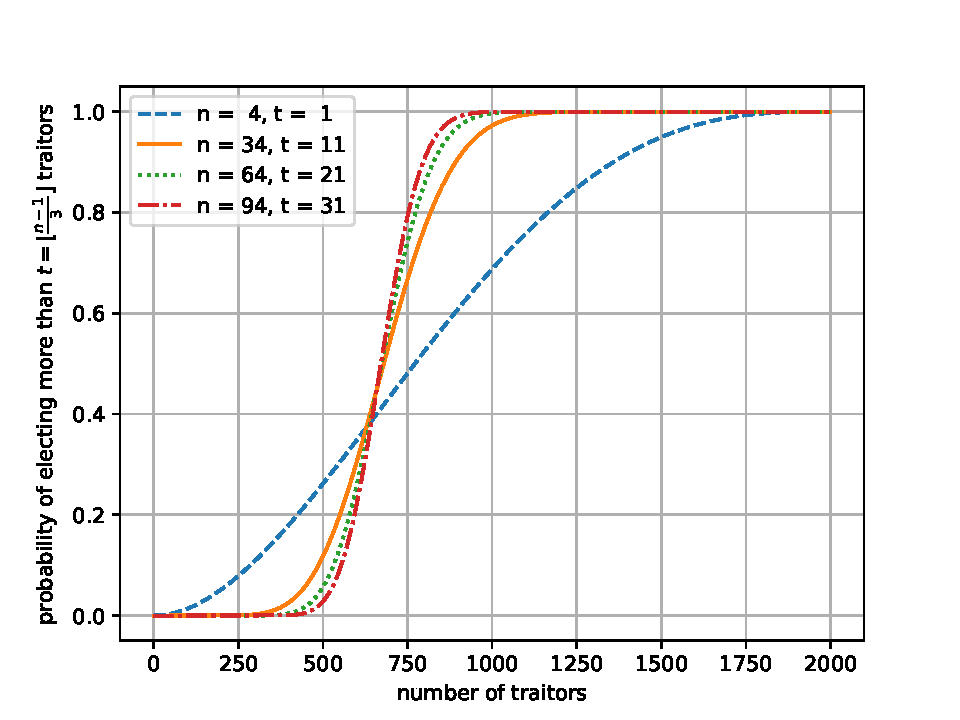
\includegraphics[width=1.0\textwidth]{hypergeometric}
  \caption{Probability of selecting more than $\lfloor \frac{n-1}{3} \rfloor$ black balls for
  different value of $t$ with $N$ fixed at 2000.}
  \label{fig:hypergeometric}
\end{figure}

On the other hand, due to the fact that hypergeometric distributions have light tails with ``faster-than-exponential fall-off''~\cite{skala2013hypergeometric},
the probability for picking more than $\lfloor \frac{n-1}{3} \rfloor$ black balls when 
the expected value is much smaller than $\lfloor \frac{n-1}{3} \rfloor$ is small.
We can use tail inequality to bound the probability of picking more than $\lfloor \frac{n-1}{3} \rfloor$ black balls when only $n\alpha$ are black where $0 \le \alpha \le \lfloor \frac{n-1}{3} \rfloor / n$.
The tail inequality is
$$
\Pr[X \ge E[X] + \tau n] \le e^{-2\tau^2n},
$$
where $E[X] = n\alpha$.
We are interested in $\Pr[X \ge \lfloor \frac{n-1}{3} \rfloor + 1]$, so
$$
\tau = \frac{\lfloor \frac{n-1}{3} \rfloor + 1}{n} - \alpha
$$
Putting $\tau$ back into the tail inequality we get the following bound.
$$
\Pr[X \ge \lfloor \frac{n-1}{3} \rfloor + 1] \le e^{-2 \big(\frac{\lfloor  \frac{n - 1}{3} \rfloor + 1}{n} - \alpha \big)^2 n}
$$

The bound is not tight, but it is useful for picking parameters for a desired level of fault tolerance.
If $n$ is fixed, since $0 \le \alpha \le \lfloor \frac{n-1}{3} \rfloor/n < (\lfloor  \frac{n - 1}{3} \rfloor + 1) / n$,
the probability is maximum when the squared term is minimum at $\alpha = \lfloor \frac{n-1}{3} \rfloor/n$.
The probability is minimum when the squared term is maximum at $\alpha = 0$.
Hence, if $n$ is known, then we can pick a $\alpha$ such that the probability becomes small.
On the other hand, if $\alpha$ is fixed, but small, we may increase $n$ to achieve the same.
To put this into perspective,
suppose $n = 100$ and $\alpha = 1/10$, i.e. 10\% of the nodes are malicious,
then the probability to draw more black balls than the threshold is $9.9 \times 10^{-6}$.

\clearemptydoublepage

\chapter{Implementation and experimental results}
\label{ch:implementation}

To build up the confidence of the horizontal scalability claim from our analytical results,
we must verify the same property experimentally.
Hence, we give an open source prototype implementation of our system.
Our implementation runs on a network with over 1000 node.
Each node sends transactions to each other autonomously, 
which allows us to evaluate our analytical claims.

We begin this chapter with a description of the implementation in \Cref{sec:implementation}.
Then, we move on to describing our experimental setup in \Cref{sec:experimental-setup} which includes a discussion on the system parameters and the physical infrastructure which we use.
Finally, \Cref{sec:comms-cost-experiment} and onwards follows the same structure as the Performance analysis (\Cref{sec:performance-analysis}),
where we analyse the performance experimentally rather than analytically and compare both results.


\section{Implementation}
\label{sec:implementation}

The prototype implementation can be found on GitHub.
\begin{displayquote}
\url{https://github.com/kc1212/consensus-thesis-code}
\end{displayquote}
It implements the three protocols and the Extended TrustChain discussed in~\Cref{ch:model}.
We also implement two optimisations---privacy preserving validation protocol using compact blocks (\Cref{sec:compact})
and optimised validation protocol using cached agreed fragments (\Cref{sec:caching}).
It is written in the event driven paradigm, using the Python programming language\footnote{\url{https://www.python.org/}}.
We use the Twisted\footnote{\url{https://twistedmatrix.com/}} library for networking.

The structure of the implementation is primarily made up of three modules---\texttt{acs}, \texttt{trustchain} and \texttt{node}.
\texttt{acs}, as its name suggests, implements ACS.
ACS uses erasure code in one of its sub-protocols (reliable broadcast).
Thus we use the liberasurecode\footnote{\url{https://github.com/openstack/liberasurecode}} library for its Reed-Solomon error correcting code functionality.
An implementation detail is that liberasurecode cannot create more than 32 code blocks\footnote{
  The 32 code blocks limitation is hardcoded in the source file, see
  \url{https://github.com/openstack/liberasurecode/blob/0794b31c623e4cede76d66be730719d24debcca9/include/erasurecode/erasurecode.h\#L35}
}, we discuss the effect of this in~\Cref{sec:experimental-setup}.
The \texttt{acs} module provides a small interface to the caller to start and stop the consensus process and also retrieve results.
The \texttt{trustchain} module implements the Extended TrustChain data structure.
It also provides the essential algorithm necessary to interact with Extended TrustChain such as 
$\textsf{new\_tx}(\cdot)$, $\textsf{new\_cp}(\cdot)$ and $\textsf{agreed\_fragment}(\cdot)$.
Finally, the \texttt{node} module ties everything together.
It implements the consensus protocol, the transaction protocol and the validation protocol.


Every node keeps a persistent TCP connection with every other node.
This creates a fully connected network for our experiment.
It is certainly not ideal in real world scenarios where nodes may have limited resources (e.g. sockets).
But as a prototype, it is sufficient to run a network of over a thousand nodes and experiment with it.

Finally, the cryptography primitives we use are SHA256 for hash functions and Ed25519 for digital signatures.
Both of which are provided by libnacl~\footnote{\url{https://pypi.python.org/pypi/libnacl}}.


\section{Experimental setup}
\label{sec:experimental-setup}

The goal of the experiment is to run the three protocols---consensus protocol,
transaction protocol and validation protocol---simultaneously and analyse the communication cost, the consensus duration and the global throughput.
We investigate these properties under the following four parameters.
\begin{enumerate}
  \item The transaction rate $r_{\text{tx}}$ per node. This is not comparable to the others because it is fixed at 2 TX/s.
        Nevertheless, it is a good value because, as we show later,
        it hits a bottleneck in extreme cases which helps us understand the limitations of our design.
  \item The number of facilitators $n \in \{4, 8, \dots, 32\}$.
        The maximum $n$ is 32 because the limitation in liberasurecode mentioned in \Cref{sec:implementation},
        but our results give a good indication of how our system may function for larger numbers of $n$.
  \item The population size $N \in \{200, 300, \dots, 1200\}$.
        $N$ stops at 1200 is due to our physical setup, which we describe next.
  \item The two modes of transaction.
        The first mode is the \emph{fixed-neighbour} mode where nodes only transact with their immediate neighbour which is predetermined. 
        This minimises the data volume per validated transaction because agreed fragment can be cached.
        The second mode is in the other extreme which we call the \emph{random-neighbour} mode,
        where every transaction is with a random node out of the $N$ nodes in the system.
        It is unlikely that the agreed fragments can be reused.
\end{enumerate}

The experiment is run on the DAS-5\footnote{\url{https://www.cs.vu.nl/das5/}}.
From now on, we use ``machines'' to refer to DAS-5 nodes and ``nodes'' to refer to a running instance in our system.
On DAS-5 we use up to 30 machines, for each machine we use up to 40 nodes.
This gives us the aforementioned 1200 number.
With this setup, we cannot run more nodes because the every machine only has 65535 ports available (minus the reserved ones).
But 40 nodes each need 1200 TCP connections which is 48000 TCP connections per machine and that is inching close to the limit.
While it is possible to have more TCP connections per machine,
but it requires additional network interface which is something we do not control on the DAS-5.
Nevertheless, running the system with 1200 nodes gives a good indication of its scalability properties as we show later.

To coordinate nodes on many different machines,
we employ a discovery server to inform every node the IP addresses and port numbers of every other node.
It is only run before the experiment and is not used during the experiment.

Finally, since Bitcoin transactions are approximately 500 bytes~\cite{txsize},
we use a uniformly random transaction size sampled between 400 and 600 bytes.


\section{Communication cost for the consensus protocol}
\label{sec:comms-cost-experiment}

The remainder of this chapter follows the same structure as the performance analysis in~\Cref{sec:performance-analysis}.
We check our analytical results experimentally and demonstrate horizontal scalability.

\begin{figure}[tb]
  \centering
  \makebox[\linewidth][c]{%
    \begin{subfigure}[b]{.7\textwidth}
      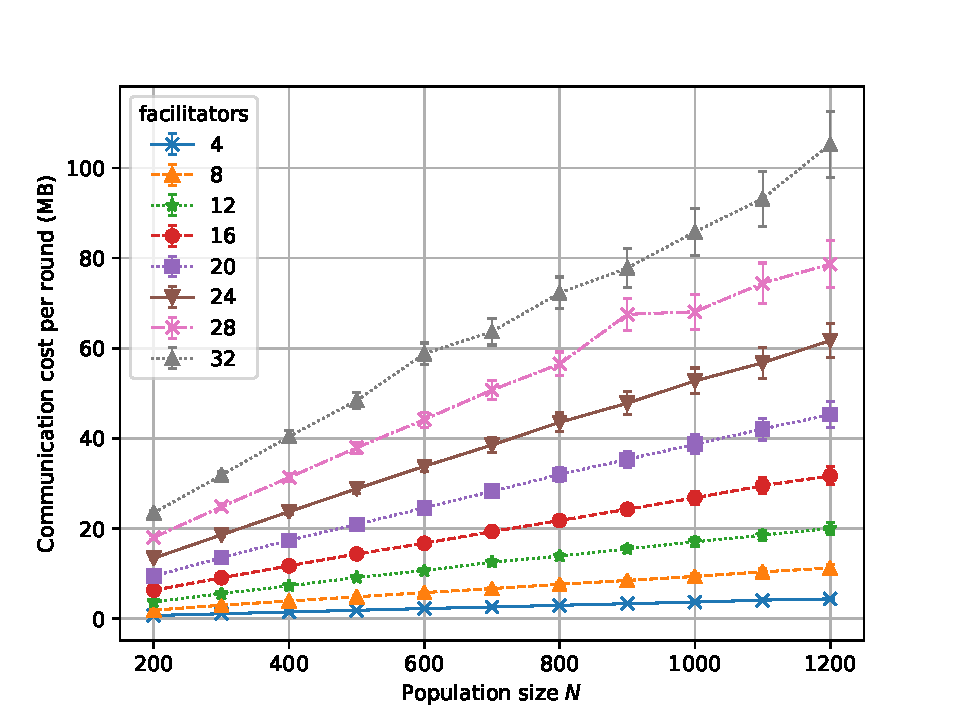
\includegraphics[width=\textwidth]{neighbour-fixed/round-communication-cost-vs-population}
      \caption{Transactions are with fixed neighbours.}
      \label{fig:round-comms-fixed}
    \end{subfigure}%
    \begin{subfigure}[b]{0.7\textwidth}
      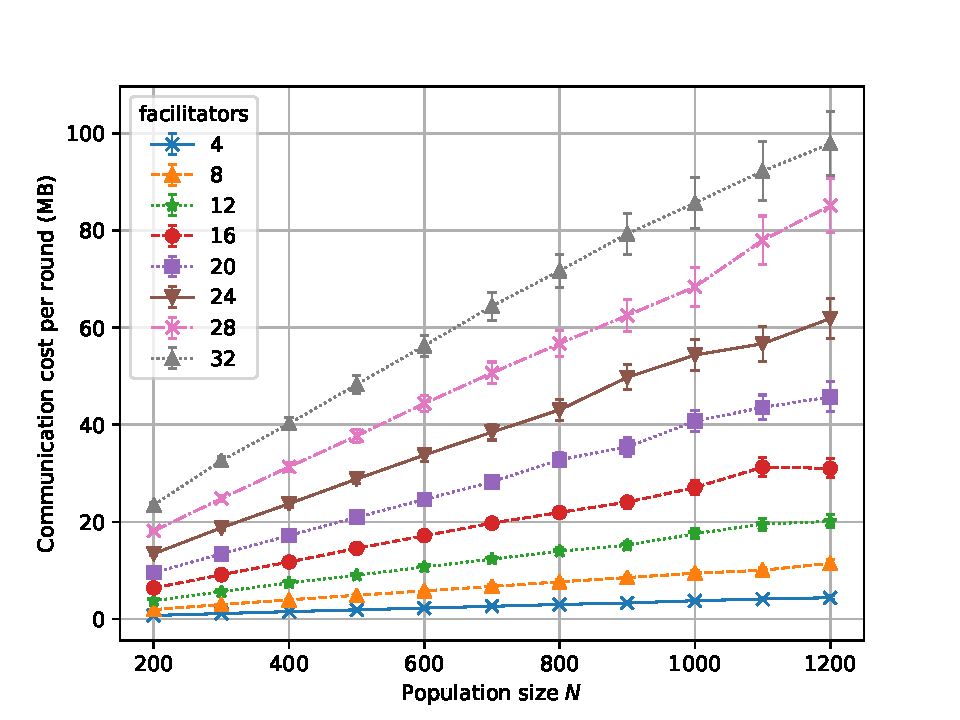
\includegraphics[width=\textwidth]{neighbour-random/round-communication-cost-vs-population}
      \caption{Transactions are with random neighbours.}
      \label{fig:round-comms-random}
    \end{subfigure}%
  }
  \caption{Communication cost for the consensus protocol per round increases linearly with population size.
  The error bars are larger for higher population size or higher number of facilitators is because rounds take longer thus they are repeated fewer times.}
  \label{fig:round-comms}
\end{figure}

\begin{figure}[tb]
  \centering
  \makebox[\linewidth][c]{%
    \begin{subfigure}[b]{.7\textwidth}
      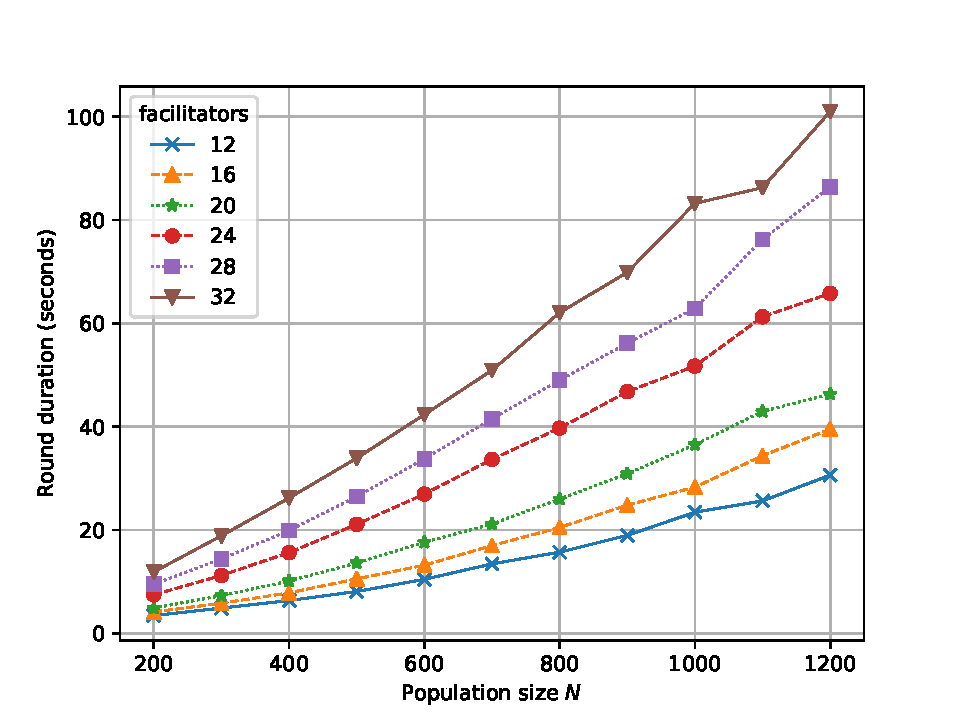
\includegraphics[width=\textwidth]{neighbour-fixed/round-duration-vs-population}
      \caption{Transactions are with fixed neighbours.}
      \label{fig:round-duration-fixed}
    \end{subfigure}%
    \begin{subfigure}[b]{0.7\textwidth}
      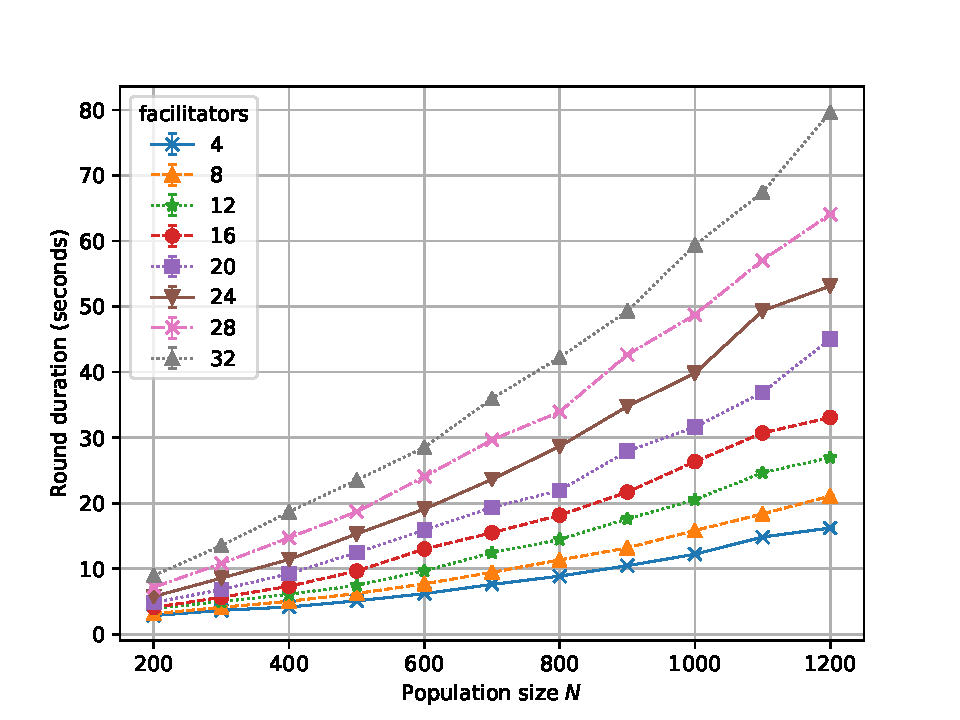
\includegraphics[width=\textwidth]{neighbour-random/round-duration-vs-population}
      \caption{Transactions are with random neighbours.}
      \label{fig:round-duration-random}
    \end{subfigure}%
  }
  \caption{Round duration does not increase linearly with the population size. 
  This is likely due to the additional hashing operation required for larger consensus result.}
  \label{fig:round-duration}
\end{figure}

\Cref{fig:round-comms} shows the relationship between the communication cost of the consensus protocol per round and the population size.
The most important aspect is that these results show a linear increase.
This reinforces our analytical result in~\Cref{sec:cons-complexity}.
Note that regardless of whether the transactions are performed with a random neighbour or with a fixed neighbour,
the magnitude of the communication cost is similar.
Both peak at about 100 MB.
This is expected because the consensus protocol is decoupled from the transaction protocol and the validation protocol.
Finally, the rate for which the communication cost increases is higher when the number of facilitators is higher.
This is also expected because the ACS algorithm has an $n^2$ term in its communication complexity.

We are also interested in how communication costs translate to time.
Hence, for the same experiment, we record the duration in seconds and the result is shown in~\Cref{fig:round-duration}.
Interestingly, the duration is not entirely linear.
We attribute this behaviour to the extra time needed to hash the CP blocks in the consensus result to compute the luck value.
Since if $N$ increases, every node must also perform more hash operations.
These results do not conform to analytical result in~\Cref{sec:cons-duration}.
Nevertheless, the difference is minor and there are ways to optimise the luck value computation.
For example, the luck value can be computed by the facilitators and are sent with the consensus result.
Then the non-facilitator nodes simply use it if there are enough signatures.

\section{Communication cost for transaction and validation protocols}

\begin{figure}[h]
  \centering
  \makebox[\linewidth][c]{%
  \begin{subfigure}[b]{0.7\textwidth}
    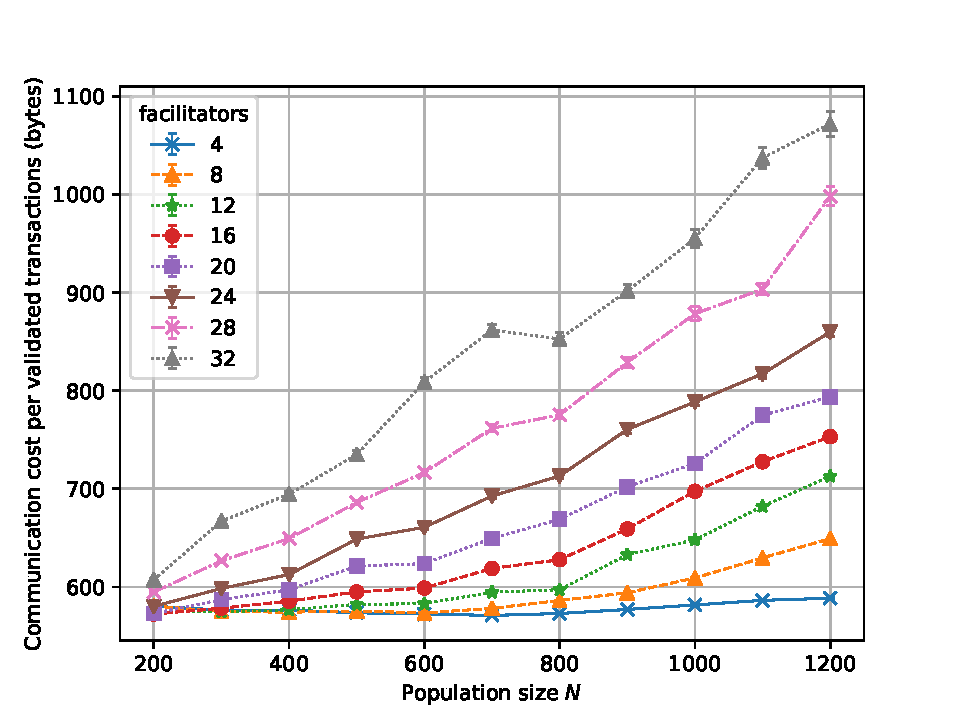
\includegraphics[width=\textwidth]{neighbour-fixed/tx-communication-cost-vs-population}
    \caption{Transactions are with fixed neighbours.}
    \label{fig:tx-comms-fixed}
  \end{subfigure}%
  \begin{subfigure}[b]{0.7\textwidth}
    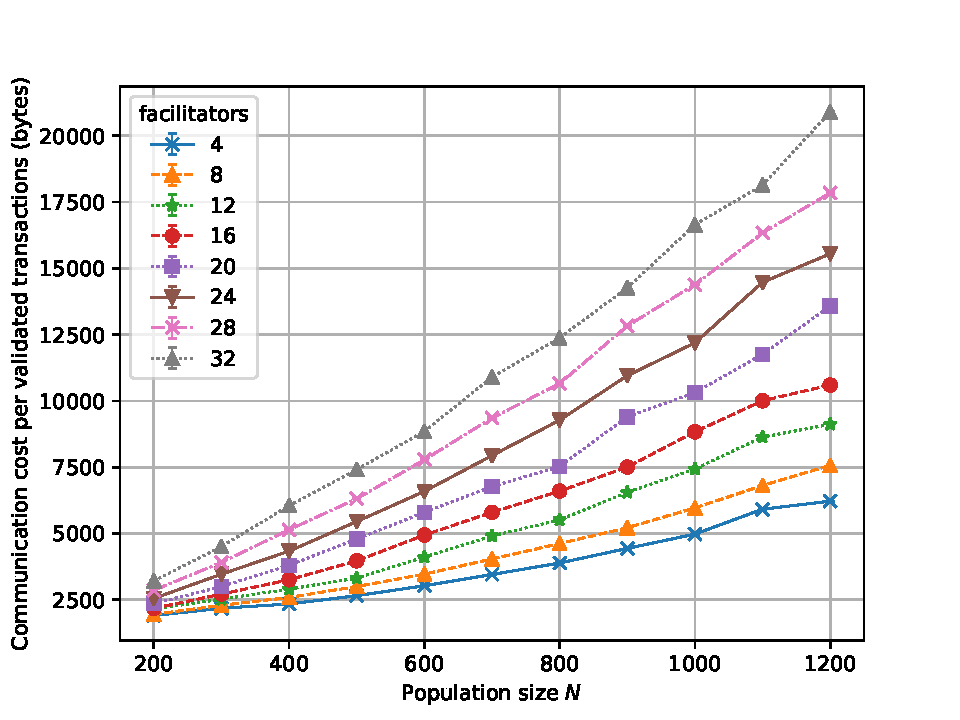
\includegraphics[width=\textwidth]{neighbour-random/tx-communication-cost-vs-population}
    \caption{Transactions are with random neighbours.}
    \label{fig:tx-comms-random}
  \end{subfigure}
  }
  \caption{Communication cost per verified transaction has similar (near linear) trend as~\Cref{fig:round-duration}.
  Fluctuation for the fixed-neighbour mode exists because the cache mechanism is unpredictable.}
  \label{fig:tx-comms}
\end{figure}

We argued that the communication cost per verified transaction is of $O(N)$ (\Cref{sec:communication-cost-for-tx}).
To verify the argument, we plot the relationship between the communication cost of for every validated transaction and population size in~\Cref{fig:tx-comms}.
We observe a near linear relationship, which is due to the near linear relationship of the communication duration mentioned before.
Again, we believe the difference is minor and it is possible to remove the extra overhead.

More interestingly, there is a large difference in communication cost between the two modes of transaction.
When transacting with only one neighbour, the communication cost is low because only one agreed fragment needs to be communicated for every round in order to validate all transactions of that round.
This is because agreed fragments are cached.
On the other hand,
if every node is transacting with a random node, then it is likely the case that one agreed fragment needs to be communicated for every transaction.
Hence the communication cost we see in~\Cref{fig:tx-comms-random} is much higher than in~\Cref{fig:tx-comms-fixed}.

Some fluctuations exist in~\Cref{fig:tx-comms-fixed}, this is due to our caching mechanism.
We send validation requests at the same rate as transactions.
Upon receiving a (remote) agreed fragment, the caching mechanism inspects all the transactions in the agreed fragment and attempts to verify as many as it can,
rather than just the transaction in the original validation request.
However, it may be the case that the agreed fragments arrive later than the validation request interval.
Then it is possible to have sent two or more validation requests for some transactions in the same local agreed fragment.
In this case, the remote would respond with two or more of the same agreed fragments,
which results in extra (wasted) communication cost, and this is the source of the fluctuation seen in~\Cref{fig:tx-comms-fixed}.
The result in~\Cref{fig:tx-comms-random} reinforces our argument.
It is a lot more stable because for every transaction it is almost always the case that an agreed fragment is needed to validate it.

\section{Linear global throughput}
\begin{figure}[h]
  \centering
  \makebox[\linewidth][c]{%
  \begin{subfigure}[b]{0.7\textwidth}
    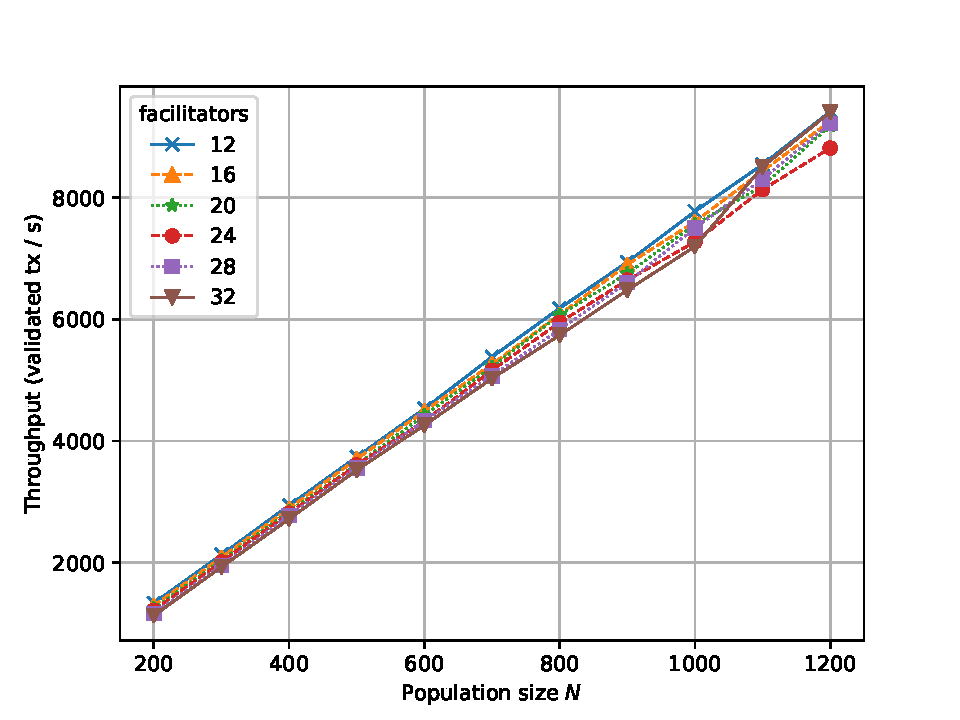
\includegraphics[width=\textwidth]{neighbour-fixed/throughput-vs-population}
    \caption{Transactions are with fixed neighbours.}
    \label{fig:global-throughput-fixed}
  \end{subfigure}%
  \begin{subfigure}[b]{0.7\textwidth}
    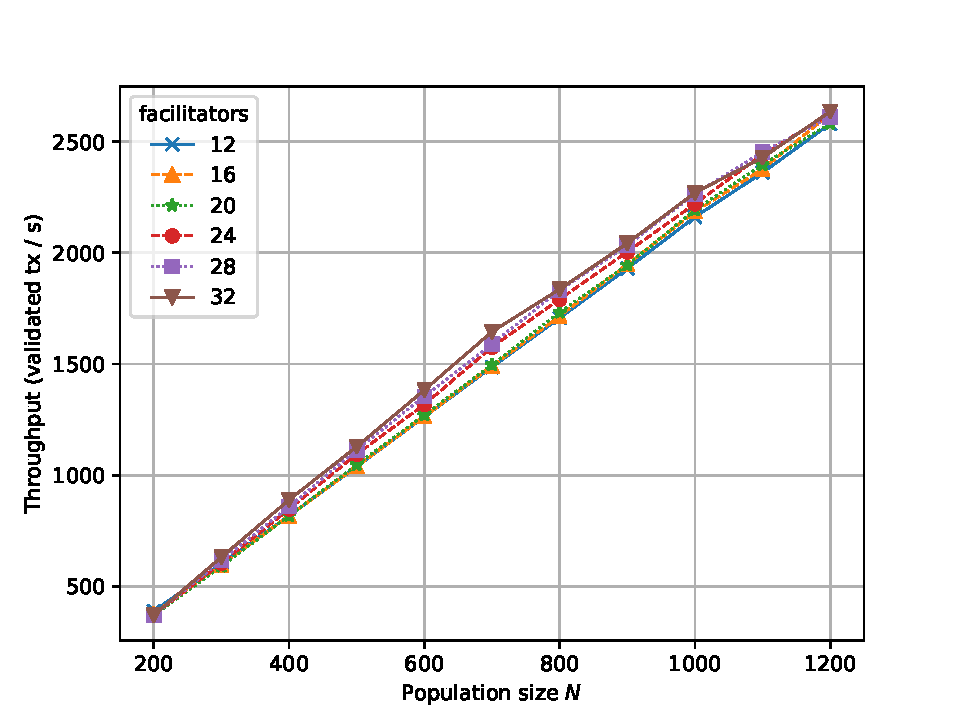
\includegraphics[width=\textwidth]{neighbour-random/throughput-vs-population}
    \caption{Transactions are with random neighbours.}
    \label{fig:global-throughput-random}
  \end{subfigure}
  }
  \caption{Global throughput increases as the population increases when every node transact at the same rate.
  Using fixed neighbours results in a higher throughput because of the caching mechanism.}
  \label{fig:global-throughput}
\end{figure}


Finally, the global throughput results are shown in~\Cref{fig:global-throughput}.
Evidently, the throughput has a linear relationship with the population size.
This result is a strong indication of the horizontal scalability which we aimed to achieve.
It also matches with our analytical result.

Note that the throughput decreases slightly as the number of facilitators increases.
This is due to the additional communication cost for running ACS with a high number of facilitators.
That is, if the network is congested then the nodes may not have enough bandwidth to send validation responses timely.

For~\Cref{fig:global-throughput-fixed},
the magnitude of our throughput may not be self-evident at first glance.
Recall that we fixed our $r_\text{tx}$ to 2, but how is it possible to have around 4800 transactions per second for 1200 nodes (which is 4 TX/s)?
This is due to the way validated transactions are calculated.
Transactions are between two parties, hence if every node makes two transactions per second,
every node also expects to receive two transactions per second.
Hence, for every node, the TX blocks are created at 4 per second.
Validation requests are sent at the same rate, which explains the magnitude.

The difference in magnitude between \Cref{fig:global-throughput-fixed} and \Cref{fig:global-throughput-random} is caused by the caching mechanism mentioned earlier.
If a new agreed fragment needs to be transmitted to validate every transaction then it puts a toll on the network infrastructure.
The low transaction rate in~\Cref{fig:global-throughput-random} is caused by the fact that the network infrastructure cannot keep up with our demand.
In practice, we do not expect such behaviour to occur as it is possible to cache agreed fragments.

We demonstrate the bottleneck issue from a different perspective in~\Cref{fig:backlog}.
The graph is plotted by counting the number of transactions and the number of validated transactions every 5 seconds for one node running in a network of 1200 nodes and 32 facilitators.
In~\Cref{fig:backlog-fixed}, the number of validated transaction changes as a step function.
This means that transactions are validated in bursts, and the validation protocol can ``keep up'' with the transactions.
Note that the horizontal ``lines'' where no new validated transactions are made are on average 76 seconds, this matches with the round duration result in~\Cref{fig:round-duration-fixed}.
On the other hand in~\Cref{fig:backlog-random}, the validation protocol clearly cannot ``keep up'' with the rate which the transactions are made.
As a result, the global throughput is lower when transacting with random nodes than only with neighbours.

\begin{figure}[tb]
  \centering
  \makebox[\linewidth][c]{%
  \begin{subfigure}[b]{0.7\textwidth}
    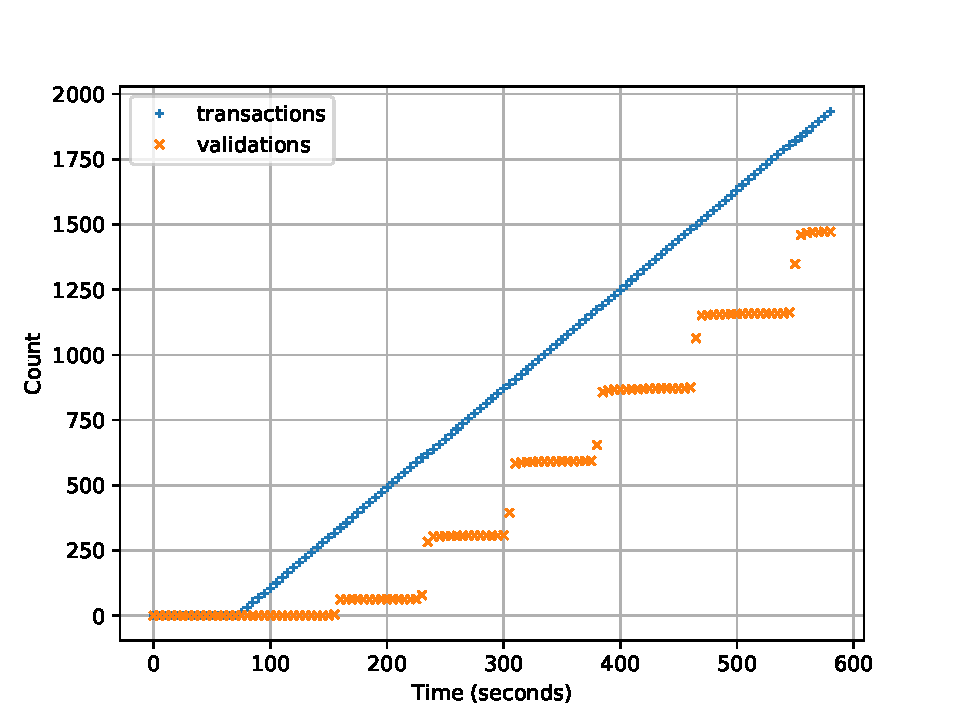
\includegraphics[width=\textwidth]{neighbour-fixed/timeseries}
    \caption{Transactions are with fixed neighbours.}
    \label{fig:backlog-fixed}
  \end{subfigure}%
  \begin{subfigure}[b]{0.7\textwidth}
    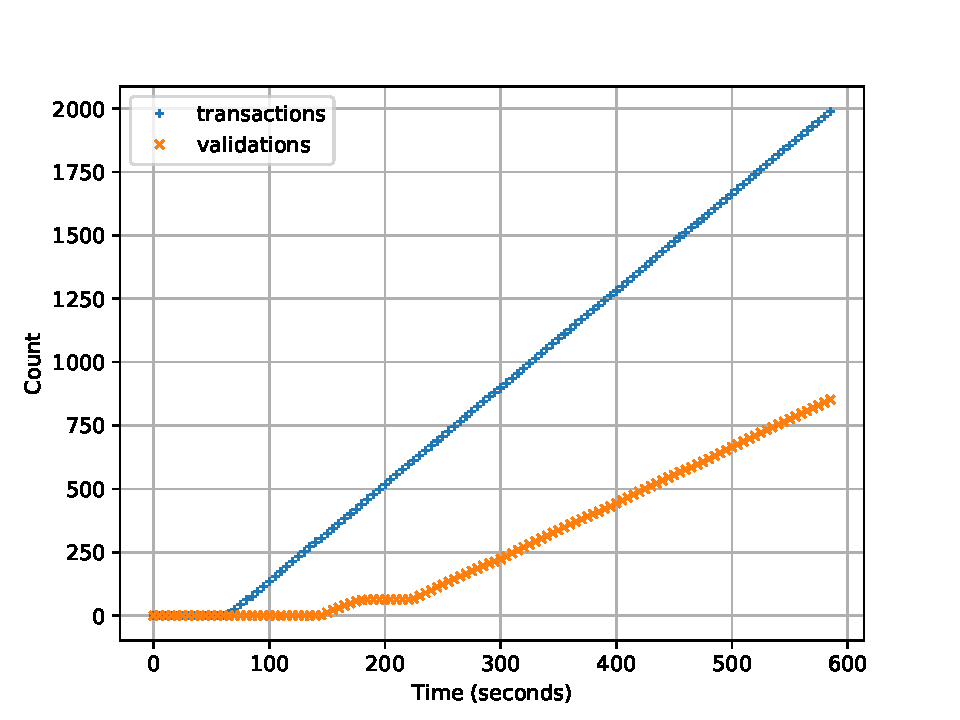
\includegraphics[width=\textwidth]{neighbour-random/timeseries}
    \caption{Transactions are with random neighbours.}
    \label{fig:backlog-random}
  \end{subfigure}
  }
  \caption{A limitation of our system is when nodes are transacting with many random nodes,
  then the network cannot keep up with the large number of agreed fragments that need to be communicated between nodes.
  Hence the slope of validated transactions grows at a slower rate in~\Cref{fig:backlog-random}.}
  \label{fig:backlog}
\end{figure}

\section{Communication cost with varying number of facilitators}
Up to this point we focused on the effect of communication cost, throughput and so on with respect to the population size.
In this section, we consider a varying number of facilitators,
which gives us an insight into our system performance may perform when the number of facilitators is higher than 32.

\begin{figure}[tb]
  \centering
  \makebox[\linewidth][c]{%
  \begin{subfigure}[b]{0.7\textwidth}
    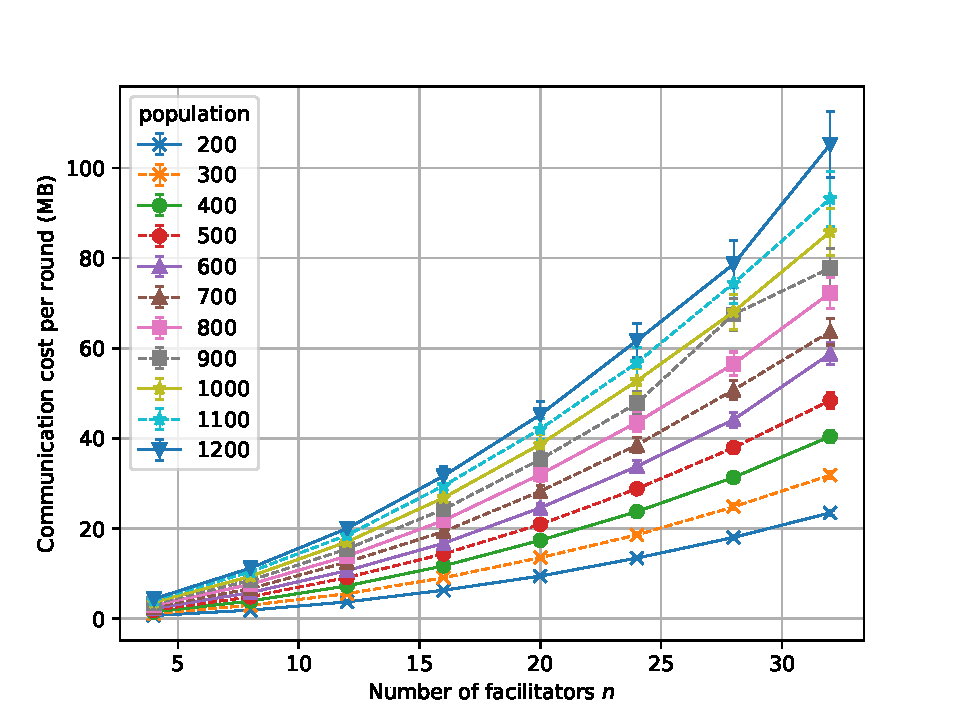
\includegraphics[width=\textwidth]{neighbour-fixed/round-communication-cost-vs-facilitators}
    \caption{Transactions are with fixed neighbours.}
    \label{fig:facilitators-round-comms-fixed}
  \end{subfigure}%
  \begin{subfigure}[b]{0.7\textwidth}
    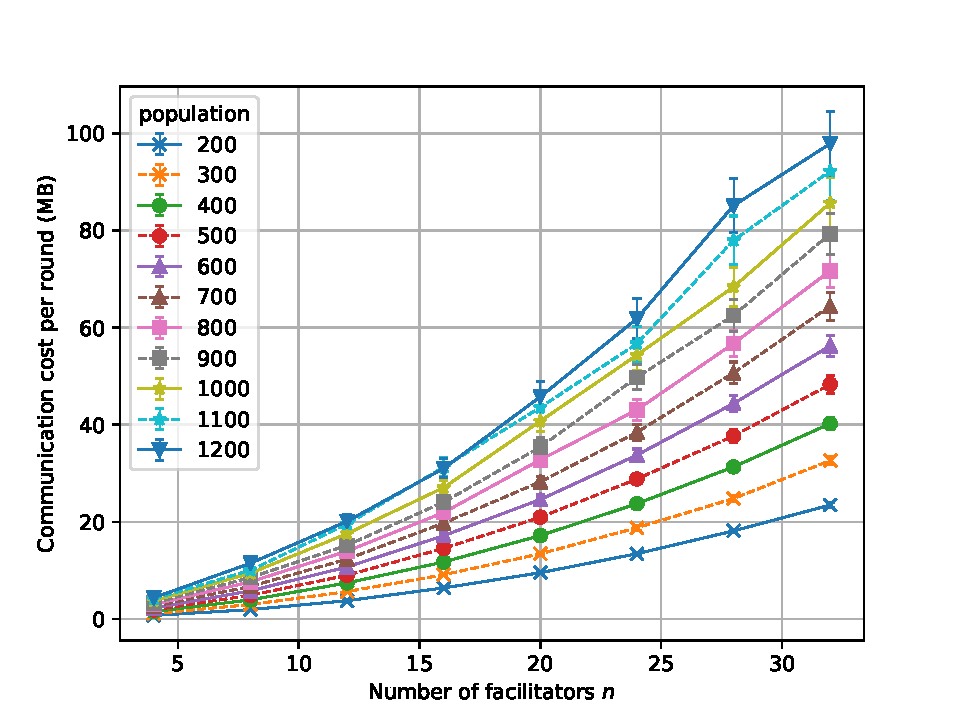
\includegraphics[width=\textwidth]{neighbour-random/round-communication-cost-vs-facilitators}
    \caption{Transactions are with random neighbours.}
    \label{fig:facilitators-round-comms-random}
  \end{subfigure}
  }
  \caption{The communication cost of the consensus protocol increases polynomially with respect to the number of facilitators as expected from the ACS communication complexity.}
  \label{fig:facilitators-round-comms}
\end{figure}

\Cref{fig:facilitators-round-comms} shows the communication cost of the consensus protocol for varying numbers of facilitators.
There is strong evidence that the communication cost grows polynomially.
We expect this because of there are polynomial terms in the ACS communication complexity---$O(n^2|v| + \lambda n^3 \log n)$.
This also means that the rounds would take longer to complete and transactions would take longer to verify.
On the other hand, we get better fault tolerance.
Thus a linear increase in fault tolerance ($t$) costs a polynomial increase in communication cost.

\clearemptydoublepage

\chapter{Related Work}
\label{ch:related}

Having analysed our system both theoretically and experimentally,
we dedicate this chapter on comparing our results with related work.
Blockchain technology has seen a surge in recent years from both the industry and academia.
We classify the various blockchain systems by their consensus approach and divide them into the following categories: 
\begin{enumerate}
    \item classical blockchain systems,
    \item classical blockchain with offchain transactions,
    \item permissioned systems,
    \item hybrid systems and
    \item blockchains without global consensus.
\end{enumerate}
A few systems from each of these categories are compared with our design.

\section{Classical Blockchain Systems}
This category represent systems with a probabilistic probabilistic consensus algorithm.
That is, transactions never reach consensus with a probability of 1.
The typical examples are proof-of-work based systems such as Bitcoin, Ethereum and other Altcoins.
In Bitcoin, the level of consensus of a block\footnote{Note that a block in Bitcoin contain many transactions whereas our TX block only contain a single transaction.}
is determined how deep it is in the Bitcoin blockchain, also called the number of confirmation.
The probability of a block being orphaned drops exponentially as the depth increases~\cite{bitcoin}.
Nevertheless, the probability of the highest block being orphaned is non-negligible.
The advantage of this type of consensus is that it can be used in a large network and is reasonably secure.
Attackers can not out pace honest users in finding new blocks unless they have a majority of the hash power.
The disadvantage however is that transactions are never in consensus with a probability of 1---no consensus finality.
Also, the performance is limited due to the fact that blocks are of fixed size and are generated at fixed intervals.

Our system significantly improves upon Bitcoin and other classical blockchain systems in performance, scalability and consensus finality.
The results described in \Cref{ch:analysis} and \Cref{ch:implementation}, show that we have horizontal scalability,
where more nodes result in more global throughput.
Further, we do not have the aforementioned probabilistic behaviour,
once some consensus result is decided, it cannot be orphaned, thus our consensus is final.
The leadership election is also not ideal in classical blockchain systems.
Mining can be seen as a technique to elect a single leader.
The leader has full control of what goes into the block thus it may selectively censor transactions.
We use ACS, so as long as the CP block is in $n - 2t$ nodes, it is guaranteed to be in consensus.

However, the security aspect falls short of the ``honest majority'' security model that classical blockchains claim to 
have\footnote{Recently it was shown that doing selfish-ming would give the adversary an unfair advantage when she only controls 25\% of the mining power~\cite{eyal2014majority}}.
Our system risks going into erroneous state if the inequality $n \ge 3t + 1$ is not satisfied.
Classical blockchain systems also have an incentive mechanism, thus they do not depend on altruistic nodes and encourages participation.
Our system on the other hand does not have an incentive mechanism because we make no assumptions on the application.

\section{Offchain Transactions}
Offchain transactions make use of the fact that, if two or more parties frequently make transactions,
then it is not necessary to store every transaction on the blockchain, only the net settlement is necessary.
The best examples are Lightning Network~\cite{lightningnetwork} and full duplex channels~\cite{decker2015fast}.
These use the Bitcoin blockchain to store the net settlement and a payment channel to conduct offchain transactions.

Offchain transaction systems are implemented using multi-signature addresses~\cite{bitcoinmultisig} and hashed time-locked Bitcoin contracts~\cite{bitcointimelock}.
If two parties wish to make transactions, they open a time-locked payment channel with a multi-signature Bitcoin address (for two parties it would be a 2-of-2 signature address).
Transactions happen off the Bitcoin blockchain and are signed by both parties.
These transactions have a timestamp and only contain the net amount since the start of the payment channel.
Before the payment channel expires, the latest of such transactions is sent to the multi-signature address.
If multiple transactions are sent to the payment channel, the latest one is used.
After payment channel is closed, the net transaction is propagated to the Bitcoin blockchain.

The advantages of such systems is that they act as add-ons to Bitcoin wish already has a large number of users.
Thus, if enough of the network wish for it (by setting a new block version),
then a large number of users will instantly benefit from it.
It also shares the advantages of Bitcoin such as security and incentives.

On the other hand, offchain transactions also suffers from the problem of Bitcoin.
Proof-of-work is still problematic as it consumes an unreasonable amount of power.
Further, sidechain transactions are limited only to an exchange of cryptocurrency,
it is less general than typical Bitcoin transactions which may be a simple smart contract.
Time-locked contracts have a strong dependency on timing, thus disputes may arise when the payment channel is just about to close.
Our system is purely asynchronous and make no assumption on timing,
in fact we assume the adversary has control of the message delivery time and order.

\section{Permissioned Systems}

This category of systems use Byzantine consensus algorithms (discussed in \Cref{sec:acs-background}).
In essence, they contain a fixed set of nodes, sometimes called validators,
that run a Byzantine consensus algorithm to decide on new blocks.
This is known as a permissioned system where the validators must be pre-determined.
Some examples include Hyperledger and Tendermint.
The consensus algorithm used in these two systems is PBFT.

A nice aspect of Byzantine consensus and in particular PBFT is that it can handle much more transactions than classical blockchain systems.
But our system has the potential to perform beyond that of PBFT because we represent many transactions with a single CP block,
enabling horizontal scalability.
Furthermore, since PBFT relies on a leader, it is not censorship resiliant.
Our system on the other hand has the benifits of ACS where CP blocks cannot be censored.
Finally, our system is able to work in the permissionless setting by simply submitting new CP blocks to the facilitators.
It can even be adapted to work in the permissioned by simply removing the luck value computation.

What we wish to have which is in Hyperledger is a smart contract system (also known as chaincodes in Hyperledger).
We hope to design and implement smart contracts by adding additional logic to the transaction protocol and the validation protocol.
Such functionalities we believe is better to be built into the backbone rather than having it as an add on.


\section{Hybrid Systems}
Hybrid systems are very recent inventions.
Just like our work, they are attempts on solving the problems of traditional blockchains.
The main characteristic of these systems is that they use a classical blockchain technique,
i.e. proof-of-work, to elect a committee and prevent Sybils.
And then they use a Byzantine consensus algorithm to actually reach consensus on a set of transactions within the committee.
Some examples are SCP~\cite{luu2015scp}, ByzCoin~\cite{kogias2016enhancing} and Solidus~\cite{abraham2016solidus}.

Our approach share many similarities with the hybrid systems.
First, we also elect a committee (facilitators) to drive consensus.
But we do not have proof-of-work for Sybil defence because we believe 
it is possible to do it efficiently, e.g. using NetFlow~\cite{pimotte}.
Secondly, our use of CP blocks and ACS is also unique.
This creates a much higher throughput and enables censorship resiliance as mentioned earlier.
For instance, ByzCoin performs just below 1000 TPS with a thousand nodes whereas we peak at 8000 TPS.

A major side effect of these hybrid systems is that they cannot guarantee correctness when there is a large number of malicious nodes.
Our system has the same issue.
For SCP, ByzCoin and Solidus, they all have some probability to elect more than $n$ Byzantine nodes into the committee.
This problem is especially difficult solve because the committee is always much smaller than the population size which has more than $t$ Byzantine nodes,
thus electing more than $t$ nodes into the committee in always a possibility.
Classical blockchain do not have this problem because they do not use Byzantine consensus.
The permissioned systems work around this problem by trusting validators.

\section{Blockchains Without Global Consensus}

Tangle~\cite{tangle}, Corda~\cite{corda} and the original TrustChain~\cite{trustchain} do not use global consensus at all.
By avoiding global consensus, they are able to achieve extreme scalability.
Just like our approach, these blockchains are also application neutral where transactions can contain arbitrary data.

Our system can be considered as the same as these types of blockchains but with a lightweight consensus protocol.
Consensus might not be applicable in all applications.
But we believe it is important for detecting and preventing fraud.
The example in~\Cref{fig:trustchain-bad} on page~\pageref{fig:trustchain-bad} demonstrates this.
If $b$ makes a fork and $a$ and $c$ have no way to communicate (e.g. the adversary may control parts of the network) ,
then $c$ is tricked to believe that her transaction with $b$ is valid.
Only when $c$ sees a conflicting chain is she able to tell that the transaction is invalid.
But $c$ does not know the true end-of-chain of $b$, thus she can never know whether her transaction is valid.
This is not possible in our system because $b$ cannot convince $c$ unless he can compute exponential time algorithms
(this is finding the second preimage for a hash function).

However, consensus and validation comes at a cost that do not exist in Tangle, Corda or the original TrustChain.
Our transaction rate is affected by the validation protocol in the worst case scenario as we saw in~\Cref{sec:evaluation}.


\clearemptydoublepage

\chapter{Conclusion}
\label{ch:conclusion}
\clearemptydoublepage

% BIBLIOGRAPHY
% \bibliographystyle{plain}
% \bibliography{references}
\printbibliography

\appendix

\chapter{Consensus protocol example}
\label{app:consensus-example}

\begin{figure}[htb]
    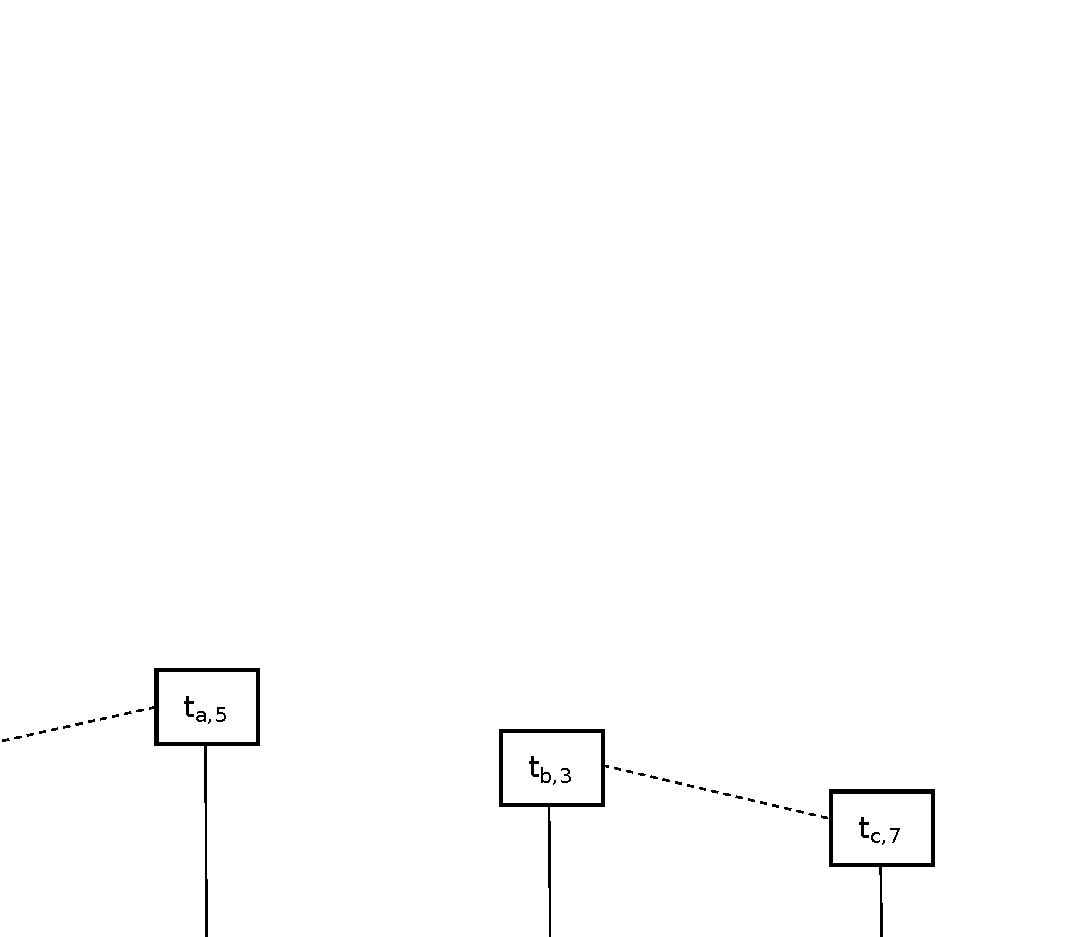
\includegraphics[trim={0 0 0 11cm}, clip, width=1.0\textwidth]{trustchain-1}
    \centering
    \caption{We begin in a state where some facilitators $\F_{r-2}$ just agreed on the consensus result $\C_{r-1}$ but have not yet propogated it yet.}
    \label{fig:trustchain-1}
\end{figure}

\begin{figure}[htb]
    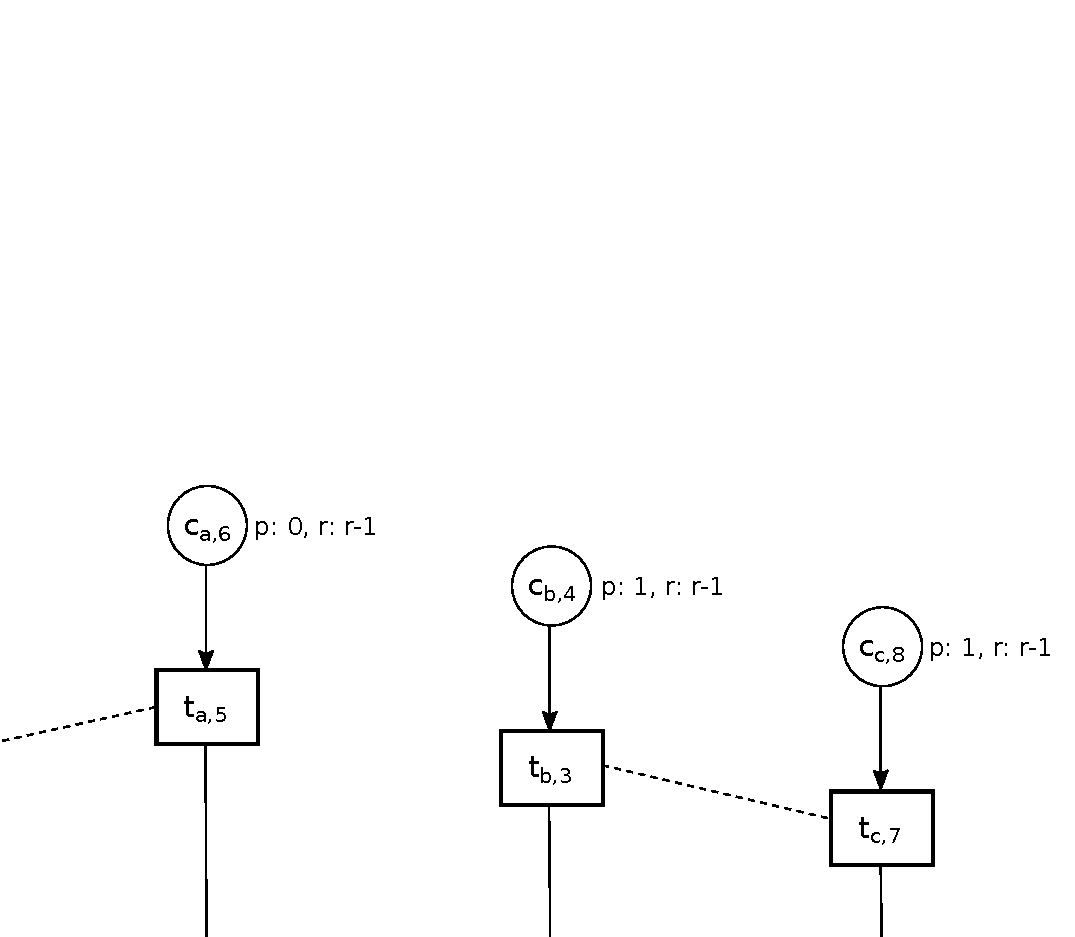
\includegraphics[trim={0 0 0 8cm}, clip, width=1.0\textwidth]{trustchain-2}
    \centering
    \caption{The facilitators propogates $\C_{r-1}$. Upon receiving it, the nodes perform two tasks;
    (1) elect new facilitators $\F_{r-1}$ by selecting the first $n$ nodes ordered by $\textsf{H}(\C_{r-1} || pk)$,
    and (2) create new CP blocks---$c_{a, 6}, c_{b, 4}$ and $c_{c, 8}$.
    $\textsf{H}(\cdot)$ is a cryptographically secure hash function and $pk$ is the public key of the respective node.}
    \label{fig:trustchain-2}
\end{figure}

\begin{figure}
    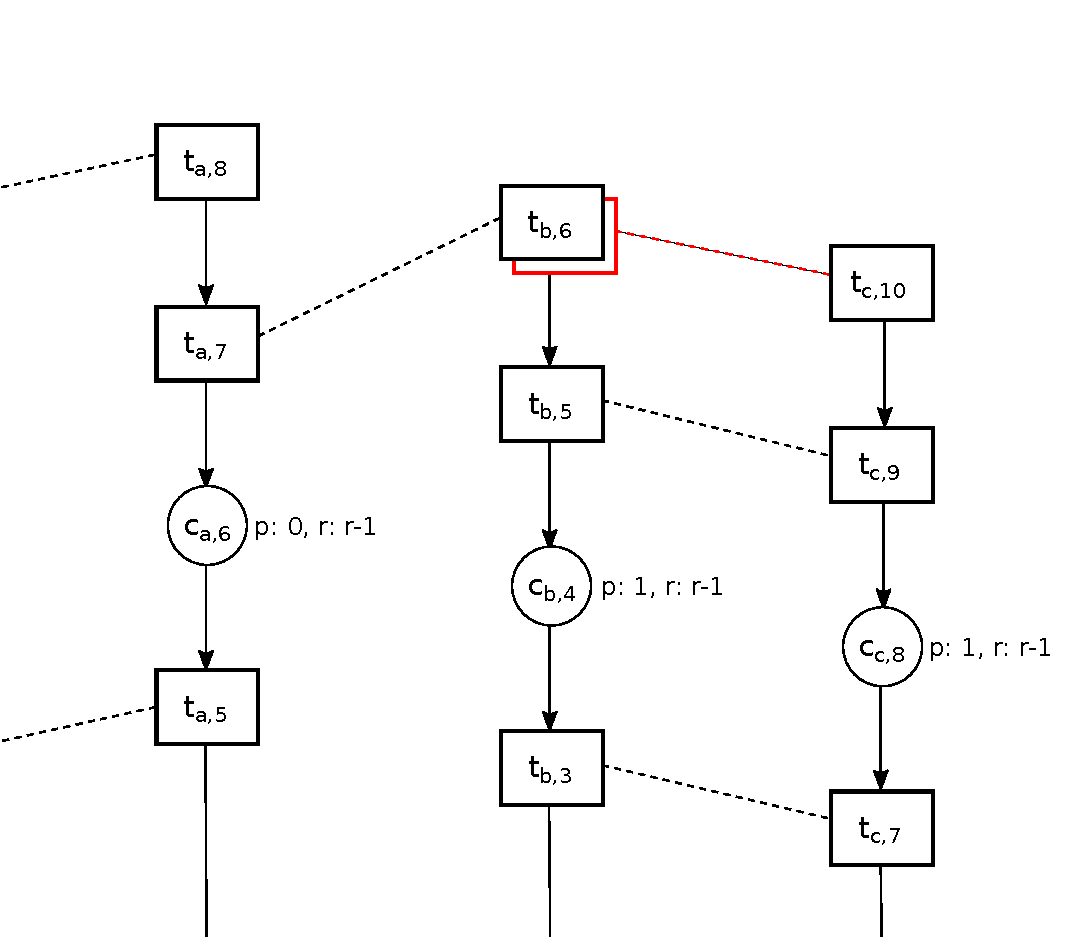
\includegraphics[trim={0 0 0 2cm}, clip, width=1.0\textwidth]{trustchain-3}
    \centering
    \caption{Nodes now send their new CP blocks to the new facilitators $\F_{r-1}$.
    While $\F_{r-1}$ is trying to reach consensus on a set of CP blocks,
    nodes carry on making transactions as usual (concurrently).
    We remark that the to-be-agreed consensus result $\C_r$ is created using CP blocks from the previous round---$c_{a, 6}, c_{b, 4}$ and $c_{c, 8}$.
    }
    \label{fig:trustchain-3}
\end{figure}

\begin{figure}
    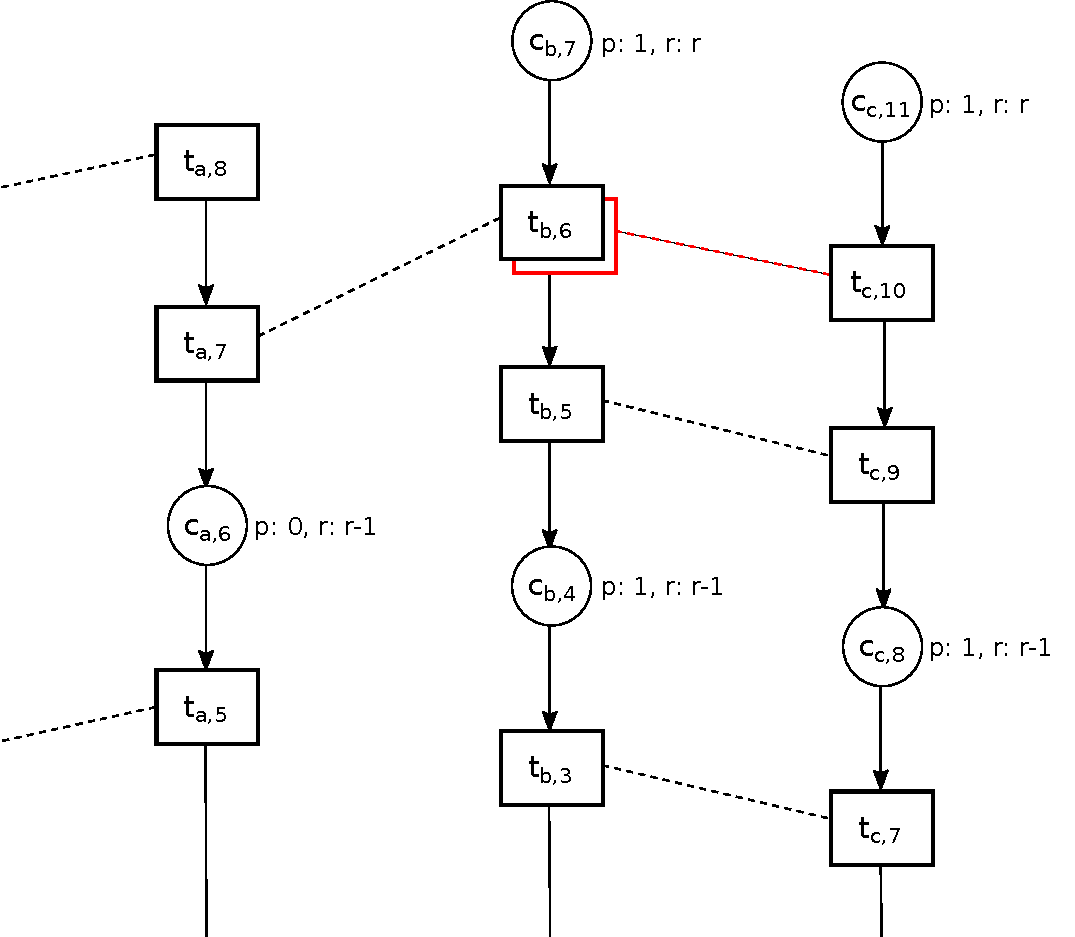
\includegraphics[width=1.0\textwidth]{trustchain-4}
    \centering
    \caption{Finally, when $\F_{r-1}$ decides on $\C_r$ (which should contain $c_{a, 6}, c_{b, 4}$ and $c_{c, 8}$) and disseminates it.
    Nodes compute new facilitators $\F_{r}$ and create new CP blocks.}
    \label{fig:trustchain-4}
\end{figure}
\clearemptydoublepage

% \chapter{Additional Graphs}
\label{app:additional-graphs}

\begin{figure}[h]
  \centering
  \begin{subfigure}{\textwidth}
    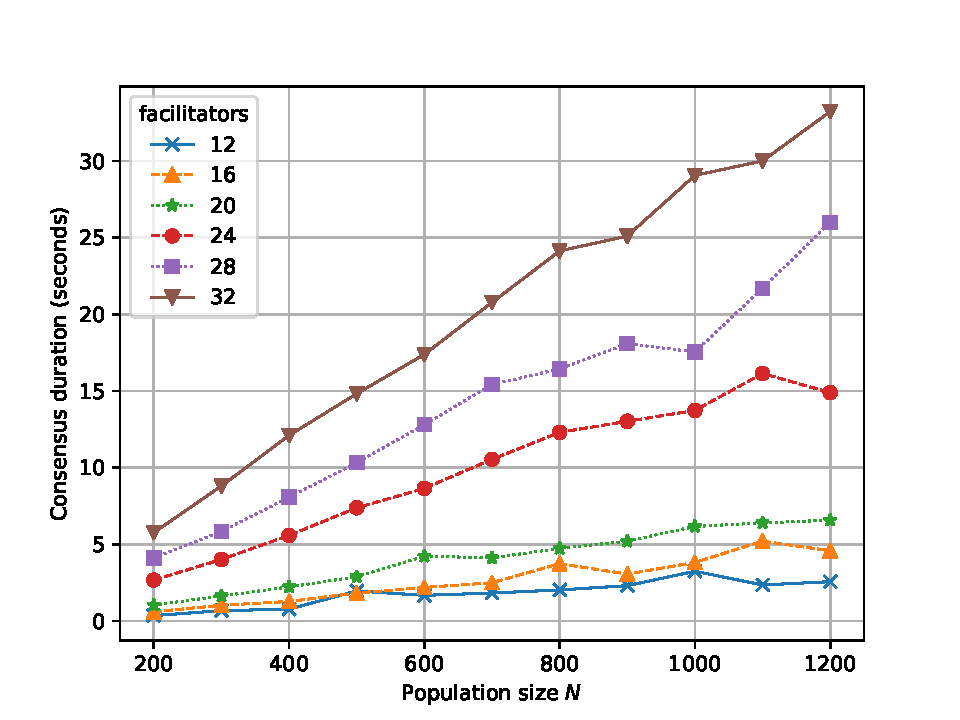
\includegraphics[width=\textwidth]{neighbour-fixed/consensus-duration-vs-population}
    \caption{Transactions are with fixed neighbours}
  \end{subfigure}

  \begin{subfigure}{\textwidth}
    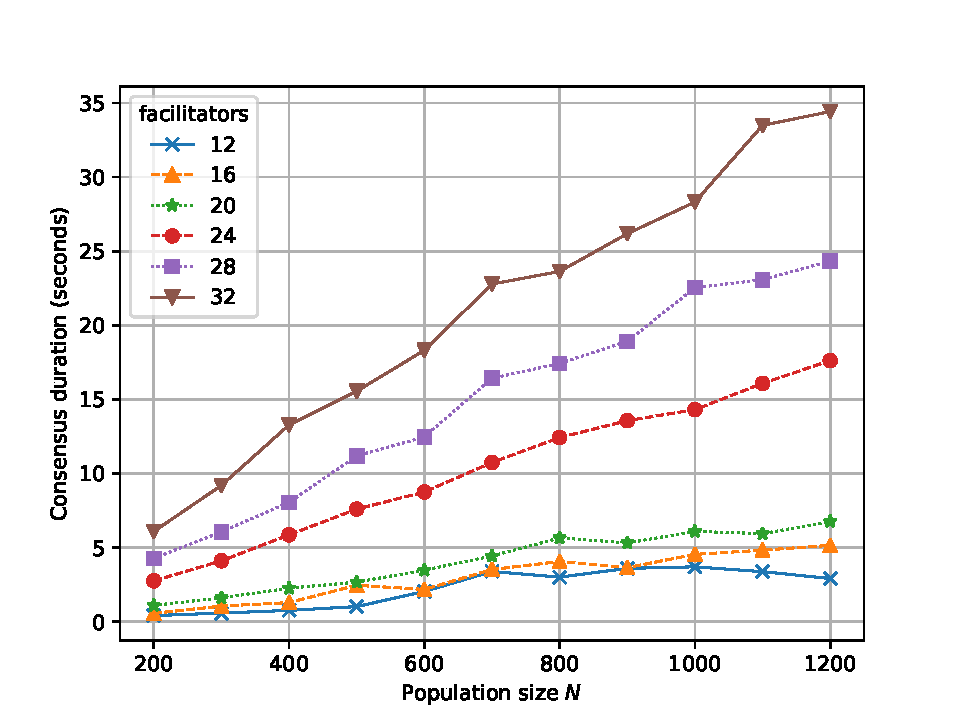
\includegraphics[width=\textwidth]{neighbour-random/consensus-duration-vs-population}
    \caption{Transactions are with random neighbours}
  \end{subfigure}
  \caption{Communication cost for consensus}
  \label{fig:consensus-duration}
\end{figure}
% \clearemptydoublepage

\end{document}

